\documentclass[a4paper,12pt]{book}
%Paquetes
\usepackage[utf8x]{inputenc}
\usepackage[spanish,activeacute,es-lcroman,es-tabla]{babel}
%\usepackage[spanish, es-tabla]{babel}
\usepackage[spanish]{minitoc}
%\usepackage{mtcoff}
%\usepackage{anttor}
\usepackage{amsmath, amsthm, amssymb}
\usepackage{amsfonts}

\usepackage{yfonts}
\usepackage{wrapfig}

%\usepackage{lettrine}
\usepackage[T1]{fontenc}
%\usepackage{lmodern}

%texlive-fontsextra
\usepackage{dsfont}
\usepackage{graphs}
\usepackage{graphicx}
\usepackage{caption}
\usepackage{subcaption}

\usepackage{pstricks} % para color
\usepackage{pst-node} % para diagramas
\usepackage{pst-plot} % para representacion de datos
                      % funciones, etc
\usepackage{pst-text}
\usepackage{pst-tree}
\usepackage{pst-circ}
\usepackage{pst-poly}
\usepackage{pstricks-add}
%\usepackage{pst-coil}
\usepackage{pst-gantt}

\usepackage{hyperref}


\usepackage{graphicx}
\usepackage{textcomp}
\usepackage{color}
\usepackage{fancyvrb}
\usepackage{fancyhdr}
\usepackage{eso-pic,calc}                        
\usepackage{bibunits}
\usepackage{listings}
\usepackage{lscape}

\usepackage{ascii}

\usepackage{anysize}

\usepackage{endnotes}

\usepackage{enumerate}





\usepackage{ascii}
\usepackage{textcomp}
\usepackage{eurosym}
\usepackage{cclicenses}

\usepackage[spanish,intoc]{nomencl}
\makenomenclature

\usepackage{makeidx}

\usepackage{filecontents}


%\TPGrid[10mm,5mm]{26}{20} 

%\parindent=0pt\chapter*{}
%\parskip=0.5\baselineskip








\let\T=\text
\fancyhead[L]{\textbf{(\textit{preview} 1.0)}} 
%\fancyhead[RE]{}
%\fancyhead[RO,LE]{\thepage}

% Utilidades
%--------------------------------------------------------------------------
\newtheorem{thm}{Teorema}[section]
\newtheorem{cor}[thm]{Corolario}
\newtheorem{lem}[thm]{Lema}
\newtheorem{prop}[thm]{Proposici\'on}
\theoremstyle{definition}
\newtheorem{defn}[thm]{Definici\'on}
\newtheorem{form}[thm]{Formalidad}
\newtheorem{regl}[thm]{Reglas}
\newtheorem{ejem}[thm]{Ejemplo}
\newtheorem{prog}[thm]{Programa}
\newtheorem{algo}[thm]{Algoritmo}
\theoremstyle{remark}
\newtheorem{rem}[thm]{Observación}
\newtheorem{dhm}[thm]{Demostración}


\let\stdthebibliography\thebibliography
\renewcommand*{\thebibliography}{%
\let\section\subsection\stdthebibliography}

\renewcommand{\notesname}{Notas}


\newcommand{\dos}{\textsf{~dos/win~}}
\newcommand{\unix}{\UNIX}
% \pdfpagewidth 6\chapter{Formalismos}
% \pdfpageheight 9in
% \setlength\topmargin{0in}
% \setlength\headheight{0in}
% \setlength\headsep{0in}
% \setlength\textheight{7.7in}
% \setlength\textwidth{6.5in}
% \setlength\oddsidemargin{0in}
% \setlength\evensidemargin{0in}
% \setlength\headheight{25pt}
% \setlength\headsep{0.25in}

\marginsize{2cm}{2cm}{2cm}{2cm} 

% \makeatletter\renewcommand\theenumii{\@roman\c@enumiii}\makeatother
% \makeatletter\renewcommand\theenumii{\@roman\c@enumii}
% \renewcommand\labelenumii{\theenumii)}
% \makeatletter % for internal macros with @
% \renewcommand\theenumii{\@roman\c@enumii}
% \makeatother

\pagestyle{empty}
\frontmatter

\setcounter{secnumdepth}{5}
\setcounter{tocdepth}{5}

\setcounter{parttocdepth}{1}
\setcounter{minitocdepth}{1}
%\nomtcrule 

\renewcommand{\mtctitle}{Resumen:}
 
%\setlength{\mtcindent}{24pt}
%\renewcommand{\mtcfont}{\texttt}
%\renewcommand{\mtcSfont}{\small\bf}

%% for Greek Alphabet

\def\X#1{$#1$ &\tt\string#1}

\definecolor{gray}{rgb}{0.98,0.98,0.98}
\definecolor{black}{rgb}{0,0,0}

\lstset{showstringspaces=false,numbers=left,
        numberstyle=\footnotesize,backgroundcolor=\color{gray},
        rulesep=1pt, rulesepcolor=\color{black},frame=leftline,
        basicstyle=\ttfamily, mathescape=true}

        
%%% Commands@dlucenap
        
        
%%%%%%%%%%%%%%%%
% Command: Double Page with style Empty
%%%%%%%%%%%%%%%%

\global\def\doublePageEmpty{\newpage{\pagestyle{empty}\cleardoublepage}}        
        
        
%%%%%%%%%%%%%%%%
% Command: Enviroment for compile chapter
% #1 name of Chapter
% #2 is a Source of file
%%%%%%%%%%%%%%%%
   
\global\def\metaChapter#1#2
{
\doublePageEmpty

\pagestyle{fancy}
% 
% \renewcommand*{\bibname}{Bibliografía capitular}
% \bibliographyunit
% \doublePageEmpty
% \bibliographyunit[\chapter]
% \bibliographystyle*{alpha}
% \bibliography*{lib}

\chapter{#1}
\minitoc
\input{#2}

\doublePageEmpty
\addcontentsline{toc}{section}{Notas}

\pagestyle{plain}

\theendnotes

\doublePageEmpty
% \addcontentsline{toc}{section}{Bibliografía capitular}
% \putbib
% \bibliographyunit

}


%%%%%%%%%%%%%%%%
% Command: Enviroment for compile chapter
% #1 name of Chapter
% #2 is a Source of file
%%%%%%%%%%%%%%%%
   
\global\def\simpleChapter#1#2
{
\doublePageEmpty

\pagestyle{fancy}
% 
% \renewcommand*{\bibname}{Bibliografía capitular}
% \bibliographyunit
% \doublePageEmpty
% \bibliographyunit[\chapter]
% \bibliographystyle*{alpha}
% \bibliography*{lib}

\chapter{#1}
\minitoc
\input{#2}

\doublePageEmpty
% \addcontentsline{toc}{section}{Notas del capítulo}
% 
% \pagestyle{plain}
% 
% \theendnotes

% \doublePageEmpty
% \addcontentsline{toc}{section}{Bibliografía capitular}
% \putbib
% \bibliographyunit

}

%%%%%%%%%%%%%%%%
% Command: 
% #1 name of Chapter
% #2 is a Source of file
%%%%%%%%%%%%%%%%
   
\global\def\preChapter#1#2
{
\doublePageEmpty
\chapter*{#1}
\input{#2}
\doublePageEmpty
}

%%%%%%%%%%%%%%%%
% Command: 
% #1 name of word
%%%%%%%%%%%%%%%%
   
\global\def\toIndex#1
{#1\index{#1} }

% \begin{filecontents*}{myStyle.xdy}
% -----------------xindy style file-----------------------
% ;;; xindy style file for the VIBS book series
% 
% ;;; xindy style file
% (markup-locclass-list :open "\dotfill" :sep "")
% 
% (define-attributes (( "textbf" "default" )) )
% (markup-locref   :attr  "textbf"     :open "\textbf{\hyperpage{" :close "}}")
% (markup-locref   :attr  "textit"     :open "\textit{\hyperpage{" :close "}}")
% (markup-locref   :attr  "textttt"     :open "\textttt{\hyperpage{" :close "}}")
% (markup-locref   :attr  "texttsc"     :open "\texttsc{\hyperpage{" :close "}}")
% (markup-locref   :attr  "default"     :open "\hyperpage{" :close "}")
% 
% define-letter-groups
%   ("a" "b" "c" "d" "e" "f" "g" "h" "i" "j" "k" "l" "m"
%    "n" "o" "p" "q" "r" "s" "t" "u" "v" "w" "x" "y" "z"))
% 
% (markup-letter-group-list :sep "~n\indexspace")
% 
% ;; End
% 
% \end{filecontents*}

\makeatletter
\renewcommand\part{%
  \if@openright
    \cleardoublepage
  \else
    \clearpage
  \fi
  \thispagestyle{empty}%   % Original »plain« replaced by »emptyx
  \if@twocolumn
    \onecolumn
    \@tempswatrue
  \else
    \@tempswafalse
  \fi
  \null\vfil
  \secdef\@part\@spart}
\makeatother

\makeindex
%\makeindex[program=texindy,columns=1]

\begin{document}

\thispagestyle{empty}
\vspace{5cm}
\begin{center}

{\LARGE
Departamento de Automática\\
Escuela Politécnica Superior\\
Universidad de Alcalá\\
}

\vspace{2cm}



\includegraphics[width=6cm]{pictures/logo-uah.eps}

\vspace{1cm}

{\LARGE \textbf{Proyecto Fin de Carrera}}

\vspace{1cm}

{\LARGE \texttt{gp1990c (GNU Pascal 1990 Compiler)}}

\vspace{2cm}

\textbf{S\v{e}ptemb\v{e}r - MMXIV}

\begin{table}[h]
\centering
\begin{tabular}{r l}
\textbf{Autor:} & Diego Antonio Lucena Pumar \\
\textbf{Titulación:} & Ingeniería Técnica en Informática de Gestión
\end{tabular}
\end{table}

\end{center}
\doublePageEmpty

%%%%%%%%%%%%%%
% Acknowledgment
%%%%%%%%%%%%%%

\preChapter{Agradecimientos}{./agradecimientos}

\doublePageEmpty

\pagestyle{plain}


%%%%%%%%%%%%%%
% Introduction
%%%%%%%%%%%%%%

%\preChapter{Prólogo}{./prologo}

%%%%%%%%%%%%%%
% Preface
%%%%%%%%%%%%%%

\preChapter{Prefacio}{./prefacio}

\doparttoc
\dominitoc
%
{\tableofcontents}
\doublePageEmpty

%
{\listoffigures}
\doublePageEmpty

%
{\listoftables}
\doublePageEmpty

\pagestyle{empty}

\begin{center}
\underline{\bf Conjuntos de Números y Operadores}
\end{center}

\begin{table}[h]
\begin{center}
\begin{tabular}{r|l}
    $\mathbb{N}$ & Conjunto de los números Naturales. \\
    $\mathbb{Z}$ & Conjunto de los números Enteros. \\ 
    $\mathbb{Q}$ & Conjunto de los números Racionales. \\
    $\mathbb{R}$, $\mathbb{R}^+$, $\mathbb{R}^n$ & Conjunto de los números Reales. \\
    $\emptyset$ & Conjunto Vacío. \\
    $\in$ & Operador de Pertenecia. \\
    $\notin$ & Operador de no Pertenecia. \\
    $\subseteq$ & Subconjunto Exclusivo. \\
    $\cup$ & Operador de Unión. \\
    $\cap$ & Operador de Intersección. \\
    $\times$ & Producto Cartersiano. \\ 
    $\wedge$ & Operador de Conjunción. \\
    $\vee$ & Operador de Disjunción. \\
    $\oplus$ & Operador OR Exclusivo. \\
    $\rightarrow$ & Operador de Implicación. \\
    $\leftrightarrow$ & Operador de Equivalencia. \\
    $\Rightarrow$ & Implicación. \\
    $\Leftarrow$ & Implicación Inversa. \\
    $\Leftrightarrow$ & Equivalencia Lógica. \\
    $\circ$ & Operador de Concatenación. \\
    $\forall$ & Cuantificador Universal. \\
    $\exists$ & Cuantificador Existencial.          
\end{tabular}
\end{center}
\end{table}

\newpage

\begin{center}
\underline{\bf Alfabeto Griego}
\end{center}

\begin{table}[h]
\begin{center}
\begin{tabular}{c|c|l}
    A & $\alpha$ & alfa  \\
    B & $\beta$ & beta \\
    $\Gamma$ & $\gamma$ & gamma \\
    $\Delta$ & $\delta$ & delta \\
    E & $\epsilon$ & epsilón\\
    Z & $\zeta$ & dseta \\
    H & $\eta$ & eta \\
    $\Theta$ & $\theta$ & zeta \\
    I & $\iota$ & iota \\
    K & $\kappa$ & cappa \\
    $\Lambda$ & $\lambda$ & lambda \\
    M & $\mu$ & my \\
    N & $\nu$ & ny \\
    $\Xi$ & $\xi$ & xi \\
    O & $o$  & omicrón \\
    $\Pi$ & $\pi$ & pi \\
    P & $\rho$ & rho \\
    $\Sigma$ & $\sigma$ & sigma \\
    T & $\tau$ & tau \\
    $\Upsilon$ & $\upsilon$ & ypsilón \\
    $\Phi$ & $\phi$ & fi \\
    X & $\chi$ & ji \\
    $\Psi$ & $\psi$ & psi \\
    $\Omega$ & $\omega$ & omega \\
\end{tabular}
\end{center}
\end{table}

\doublePageEmpty

\mainmatter

%%%%%%%%%%%%%%
% PART ONE
%%%%%%%%%%%%%%

\part{Introducción}
\doublePageEmpty

% Poema: Ideario, Francisco M. Ortega Palomares.
\addstarredchapter{Francisco M. Ortega Palomares. \textit{Ideario}}
\begin{verse}

\begin{center}

\underline{\bf Ideario}

Me da vértigo el punto muerto \\

y la marcha atrás, \\

vivir en los atascos, \\

los frenos automáticos y el olor a gasoil.

\par

Me angustia el cruce de miradas \\

la doble dirección de las palabras \\

y el obsceno guiñar de los semáforos.

\par

Me da pena la vida, los cambios de sentido, \\

las señales de stop y los pasos perdidos.

\par

Me agobian las medianas, \\

las frases que están hechas, \\

los que nunca saludan y los malos profetas.

\par

Me fatigan los dioses bajados del Olimpo \\

a conquistar la Tierra \\

y los necios de espíritu.

\par

Me entristecen quienes me venden clines \\

en los pasos de cebra, \\

los que enferman de cáncer \\

y los que sólo son simples marionetas.

\par

Me aplasta la hermosura \\

de los cuerpos perfectos, \\

las sirenas que ululan en las noches de fiesta, \\

los códigos de barras, \\

el baile de etiquetas.

\par

Me arruinan las prisas y las faltas de estilo, \\

el paso obligatorio, las tardes de domingo \\

y hasta la línea recta.

\par

Me enervan los que no tienen dudas \\

y aquellos que se aferran \\

a sus ideales sobre los de cualquiera.



Me cansa tanto tráfico \\

y tanto sinsentido, \\

parado frente al mar mientras que el mundo gira.

\par{\it Francisco M. Ortega Palomares}

\end{center}

\end{verse}           
\doublePageEmpty

%%%%%%%%%%%%%%
% Chapter 1
%%%%%%%%%%%%%%

\metaChapter{Formalismos}{./parte1/capitulo1/cap1}

%%%%%%%%%%%%%%
% Chapter 2
%%%%%%%%%%%%%%

\metaChapter{Resumen: Proyecto {\tt gp1990c}}{./parte1/capitulo2/cap2}

%%%%%%%%%%%%%%
% Chapter 3
%%%%%%%%%%%%%%

\metaChapter{El Lenguaje de Programaci\'on Pascal}{./parte1/capitulo3/cap3}

%%%%%%%%%%%%%%
% Chapter 4
%%%%%%%%%%%%%%

\metaChapter{Compiladores del Lenguaje Pascal}{./parte1/capitulo4/cap4}

%%%%%%%%%%%%%%
% PART TWO: LEX
%%%%%%%%%%%%%%

\part{{\tt gp1990la} (Analizador Léxico)}
%% Poema: XI, Gustavo Adolfo Bécquer.
\pagestyle{empty}
\addstarredchapter{Gustavo Adolfo Bécquer. \textit{XI}}
\begin{verse}

\begin{center}

\underline{\bf XI}


Yo sé un himno gigante y extraño \\


que anuncia en la noche del alma una aurora, \\


y estas páginas son de ese himno \\


cadencias que el aire dilata en las sombras.

\par

Yo quisiera escribirle, del hombre \\


domando el rebelde mezquino idioma, \\


con palabras que fuesen a un tiempo \\


suspiros y risas, colores y notas.

\par


Pero en vano es luchar; que no hay cifra \\


capaz de encerrarle, y apenas ¡oh! ¡hermosa! \\


si teniendo en mis manos las tuyas \\


pudiera al oído cantártelo a solas.

\par{\it Gustavo Adolfo Bécquer}

\end{center}

\end{verse}      
\doublePageEmpty

%%%%%%%%%%%%%%
% Chapter 5
%%%%%%%%%%%%%%

\metaChapter{Formalidades del Analizador L\'exico}{./parte2/capitulo1/cap1}

%%%%%%%%%%%%%%
% PART TREE: YACC
%%%%%%%%%%%%%%

\part{{\tt gp1990sa} (Analizador Sintáctico)}
%% Poema: Retrato, Antonio Machado.
\pagestyle{empty}
\addstarredchapter{Antonio Machado. \textit{Retrato}}
\begin{verse}

\begin{center}

\underline{\bf Retrato}

Mi infancia son recuerdos de un patio de Sevilla, \\


y un huerto claro donde madura el limonero; \\


mi juventud, veinte años en tierras de Castilla; \\


mi historia, algunos casos que recordar no quiero.

\par

Ni un seductor Mañara, ni un Bradomín he sido \\


¿ya conocéis mi torpe aliño indumentario?, \\


más recibí la flecha que me asignó Cupido, \\


y amé cuanto ellas puedan tener de hospitalario.

\par

Hay en mis venas gotas de sangre jacobina, \\


pero mi verso brota de manantial sereno; \\


y, más que un hombre al uso que sabe su doctrina, \\


soy, en el buen sentido de la palabra, bueno.

\par

Adoro la hermosura, y en la moderna estética \\


corté las viejas rosas del huerto de Ronsard; \\


mas no amo los afeites de la actual cosmética, \\


ni soy un ave de esas del nuevo gay-trinar.

\par

Desdeño las romanzas de los tenores huecos \\


y el coro de los grillos que cantan a la luna. \\


A distinguir me paro las voces de los ecos, \\


y escucho solamente, entre las voces, una.

\par

¿Soy clásico o romántico? No sé. Dejar quisiera \\


mi verso, como deja el capitán su espada: \\


famosa por la mano viril que la blandiera, \\


no por el docto oficio del forjador preciada.

\par

Converso con el hombre que siempre va conmigo \\


¿quien habla solo espera hablar a Dios un día?; \\


mi soliloquio es plática con ese buen amigo \\


que me enseñó el secreto de la filantropía.

\par

Y al cabo, nada os debo; debéisme cuanto he escrito. \\


A mi trabajo acudo, con mi dinero pago \\


el traje que me cubre y la mansión que habito, \\


el pan que me alimenta y el lecho en donde yago.

\par

Y cuando llegue el día del último vïaje, \\


y esté al partir la nave que nunca ha de tornar, \\


me encontraréis a bordo ligero de equipaje, \\


casi desnudo, como los hijos de la mar.

\par{\it Antonio Machado}

\end{center}

\end{verse}      
\doublePageEmpty

%%%%%%%%%%%%%%
% Chapter 9
%%%%%%%%%%%%%%

\metaChapter{Formalidades del Analizador Sintactico}{./parte3/capitulo1/cap1}

%%%%%%%%%%%%%%
% PART FOUR: TEST
%%%%%%%%%%%%%%

%\part{Pruebas}
%\doublePageEmpty

%%%%%%%%%%%%%%
% Chapter 11
%%%%%%%%%%%%%%

%\metaChapter{Eficiencia y Optimizaci\'on}{./parte4/capitulo1/cap1}

%%%%%%%%%%%%%%
% PART FIVE: APPENDS
%%%%%%%%%%%%%%

\part{Anexos y Formalidades}
%% Poema:.
\pagestyle{empty}
%\addstarredchapter{Antonio Machado. \textit{Retrato}}
%\begin{verse}

\begin{center}

\underline{\bf Retrato}

Mi infancia son recuerdos de un patio de Sevilla, \\


y un huerto claro donde madura el limonero; \\


mi juventud, veinte años en tierras de Castilla; \\


mi historia, algunos casos que recordar no quiero.

\par

Ni un seductor Mañara, ni un Bradomín he sido \\


¿ya conocéis mi torpe aliño indumentario?, \\


más recibí la flecha que me asignó Cupido, \\


y amé cuanto ellas puedan tener de hospitalario.

\par

Hay en mis venas gotas de sangre jacobina, \\


pero mi verso brota de manantial sereno; \\


y, más que un hombre al uso que sabe su doctrina, \\


soy, en el buen sentido de la palabra, bueno.

\par

Adoro la hermosura, y en la moderna estética \\


corté las viejas rosas del huerto de Ronsard; \\


mas no amo los afeites de la actual cosmética, \\


ni soy un ave de esas del nuevo gay-trinar.

\par

Desdeño las romanzas de los tenores huecos \\


y el coro de los grillos que cantan a la luna. \\


A distinguir me paro las voces de los ecos, \\


y escucho solamente, entre las voces, una.

\par

¿Soy clásico o romántico? No sé. Dejar quisiera \\


mi verso, como deja el capitán su espada: \\


famosa por la mano viril que la blandiera, \\


no por el docto oficio del forjador preciada.

\par

Converso con el hombre que siempre va conmigo \\


¿quien habla solo espera hablar a Dios un día?; \\


mi soliloquio es plática con ese buen amigo \\


que me enseñó el secreto de la filantropía.

\par

Y al cabo, nada os debo; debéisme cuanto he escrito. \\


A mi trabajo acudo, con mi dinero pago \\


el traje que me cubre y la mansión que habito, \\


el pan que me alimenta y el lecho en donde yago.

\par

Y cuando llegue el día del último vïaje, \\


y esté al partir la nave que nunca ha de tornar, \\


me encontraréis a bordo ligero de equipaje, \\


casi desnudo, como los hijos de la mar.

\par{\it Antonio Machado}

\end{center}

\end{verse}      
\doublePageEmpty

% Style
\appendix

%%%%%%%%%%%%%%
% APPEND A: Blaise Pascal
%%%%%%%%%%%%%%

\pagestyle{plain}
\chapter{Blaise Pascal}
\label{chap:blaisePascal}

% \begin{figure}[t]
%  \centering
%  \includegraphics{./images/blaisePascal50pc.eps}
%  % Blaise_pascal.eps: 0x0 pixel, 300dpi, 0.00x0.00 cm, bb=-0 -0 299 313
%  \label{fig:Blaise Pascal}
% \end{figure}

\begin{flushright}
\textit{``El corazón tiene razones que la razón ignora.''}
\end{flushright}


{

\yinipar{B}laise Pascal\index{Blaise Pascal}, nacido el 19 de Junio de 1623 en Clemont y fallecido el 19 de Agosto de 1662 en París, es un importantísimo pensador: matemático físico, filósofo y escritor. Podemos afirmar que es ``un hombre e su época...''.
Pascal fue un importante racionalista a la vez que, según el paso de los años dedico enormes esfuerzos en ``racionalizar'' el Cristianismo y la figura e Dios. Es considerado un importante teólogo.

}

Trabajó en el campo de las matemáticas y diseño una máquina de cálculo ``Pascalina\index{Pascalina}'' capaz de realizar adiciones, con el tiempo, la propia máquina incorporó la operación de substracción.


Entre su más destacables estudios se encuentra la demostración del vació. \textit{Traité sur le vide} (Tratado sobre el vacío).


\paragraph*{Bibliografía:}
\begin{enumerate}[i.]
\item \textit{Essai pour les coniques} (1639) 
\item \textit{Experiences nouvelles touchant le vide} (1647)
\item \textit{Traité du triangle arithmétique} (1653)
\item \textit{Lettres provinciales} (1656–57)
\item \textit{De l'Esprit géométrique} (1657 o 1658)
\item \textit{Écrit sur la signature du formulaire} (1661)
\item \textit{Pensées} (Sin terminar)
\end{enumerate}



\doublePageEmpty

%%%%%%%%%%%%%%
% APPEND B: Grammars
%%%%%%%%%%%%%%

%// Generated by gramex V2.1 from 'iso_pascal_7185.txt' on Jan 25 2007 at 11:56:25
%// Command line: C:\elsie\lag\grammars\pascal\gramex.exe -p -c iso_pascal_7185.txt

\chapter{gp1990sa.y}
\label{chap:grammars}

\section{Yacc}

%// Generated by gramex V2.1 from 'iso_pascal_7185.txt' on Jan 25 2007 at 11:56:25
%// Command line: C:\elsie\lag\grammars\pascal\gramex.exe -p -c iso_pascal_7185.txt

\chapter{gp1990sa.y}
\label{chap:grammars}

\section{Yacc}

%// Generated by gramex V2.1 from 'iso_pascal_7185.txt' on Jan 25 2007 at 11:56:25
%// Command line: C:\elsie\lag\grammars\pascal\gramex.exe -p -c iso_pascal_7185.txt

\chapter{gp1990sa.y}
\label{chap:grammars}

\section{Yacc}

\input{./grammars/grammars31/gp1990sa}






\doublePageEmpty


%%%%%%%%%%%%%%
% APPEND B: Grammars
%%%%%%%%%%%%%%

%// Generated by gramex V2.1 from 'iso_pascal_7185.txt' on Jan 25 2007 at 11:56:25
%// Command line: C:\elsie\lag\grammars\pascal\gramex.exe -p -c iso_pascal_7185.txt

\chapter{Gramáticas}
\label{chap:grammars}

\section{Pascal ISO 1990:7185}

% \renewcommand{\theFancyVerbLine}{% 
% \textcolor{gray}
% {\small
% ps.\arabic{FancyVerbLine}}}

\renewcommand{\theFancyVerbLine}{%
{\small
ps.\arabic{FancyVerbLine}}}
 \begin{Verbatim}[numbers=left]
<program> ::= program <identifier> ; <block> . <identifier> ::= <letter >

{<letter or digit>}

<letter or digit> ::= <letter> | <digit>

<block> ::= <label declaration part> <constant definition part> <type definition
part> <variable declaration part>

<procedure and function declaration part> <statement part>

<label declaration part> ::= <empty> | label <label> {, <label>} ;

<label> ::= <unsigned integer>

<constant definition part> ::= <empty> | const <constant definition> { ;
<constant definition>} ; <constant definition> ::= <identifier> = <constant>
<constant> ::= <unsigned number> | <sign> <unsigned number> | <constant
identifier> | <sign> <constant identifier> |

<string>

<unsigned number> ::= <unsigned integer> | <unsigned real>

<unsigned integer> ::= <digit> {<digit>}

<unsigned real> ::= <unsigned integer> . <unsigned integer> | <unsigned integer>
. 

<unsigned integer> E <scale factor>|

<unsigned integer> E <scale factor>

<scale factor> ::= <unsigned integer> | <sign> <unsigned integer>

<sign> ::= + | -

<constant identifier> ::= <identifier>

<string> ::= '<character> {<character>}'

<type definition part> ::= <empty> | type <type definition> {;<type
definition>};

<type definition> ::= <identifier> = <type>

<type> ::= <simple type> | <structured type> | <pointer type>

<simple type> ::= <scalar type> | <subrange type> | <type identifier>

<scalar type> ::= (<identifier> {,<identifier>})

<subrange type> ::= <constant> .. <constant>

<type identifier> ::= <identifier>

<structured type> ::= <array type> | <record type> | <set type> | <file type>

<array type> ::= array [<index type>{,<index type>}] of <component type>

<index type> ::= <simple type>

<component type> ::= <type>

<record type> ::= record <field list> end

<field list> ::= <fixed part> | <fixed part> ; <variant part> | <variant part>

<fixed part> ::= <record section> {;<record section>}

<record section> ::= <field identifier> {, <field identifier>} : <type> |
<empty>

<variant type> ::= case <tag field> <type identifier> of <variant> { ;
<variant>}

<tag field> ::= <field identifier> : | <empty>

<variant> ::= <case label list> : ( <field list> ) | <empty>

<case label list> ::= <case label> {, <case label>}

<case label> ::= <constant>

<set type> ::=set of <base type>

<base type> ::= <simple type>

<file type> ::= file of <type>

<pointer type> ::= <type identifier>

<variable declaration part> ::= <empty> | var <variable declaration> {;
<variable declaration>} ;

<variable declaration> ::= <identifier> {,<identifier>} : <type>

<procedure and function declaration part> ::= {<procedure or function
declaration > ;}

<procedure or function declaration > ::= <procedure declaration > | <function
declaration >

<procedure declaration> ::= <procedure heading> <block>

<procedure heading> ::= procedure <identifier> ; |

procedure <identifier> ( <formal parameter section> {;<formal parameter
section>} );

<formal parameter section> ::= <parameter group> | var <parameter group> |

function <parameter group> | procedure <identifier> { , <identifier>}

<parameter group> ::= <identifier> {, <identifier>} : <type identifier>

<function declaration> ::= <function heading> <block>

<function heading> ::= function <identifier> : <result type> ; |

function <identifier> ( <formal parameter section> {;<formal parameter section>}
) : <result type> ;

<result type> ::= <type identifier>

<statement part> ::= <compund statement>

<statement> ::= <unlabelled statement> | <label> : <unlabelled statement>

<unlabelled statement> ::= <simple statement> | <structured statement>

<simple statement> ::= <assignment statement> | <procedure statement> | <go to
statement> | <empty statement>

<assignment statement> ::= <variable> := <expression> | <function identifier> :=
<expression>

<variable> ::= <entire variable> | <component variable> | <referenced variable>

<entire variable> ::= <variable identifier>

<variable identifier> ::= <identifier>

<component variable> ::= <indexed variable> | <field designator> | <file buffer>

<indexed variable> ::= <array variable> [<expression> {, <expression>}]

<array variable> ::= <variable>

<field designator> ::= <record variable> . <field identifier>

<record variable> ::= <variable>

<field identifier> ::= <identifier>

<file buffer> ::= <file variable>

<file variable> ::= <variable>

<referenced variable> ::= <pointer variable>

<pointer variable> ::= <variable>

<expression> ::= <simple expression> | <simple expression> <relational operator>
<simple expression>

<relational operator> ::= = | <> | < | <= | >= | > | in

<simple expression> ::= <term> | <sign> <term>| <simple expression> <adding
operator> <term>

<adding operator> ::= + | - | or

<term> ::= <factor> | <term> <multiplying operator> <factor>

<multiplying operator> ::= * | / | div | mod | and

<factor> ::= <variable> | <unsigned constant> | ( <expression> ) | <function
designator> | <set> | not <factor>

<unsigned constant> ::= <unsigned number> | <string> | < constant identifier> <
nil>

<function designator> ::= <function identifier> | <function identifier ( <actual
parameter> {, <actual parameter>} )

<function identifier> ::= <identifier>

<set> ::= [ <element list> ]

<element list> ::= <element> {, <element> } | <empty>

<element> ::= <expression> | <expression> .. <expression>

<procedure statement> ::= <procedure identifier> | <procedure identifier>
(<actual parameter> {, <actual parameter> })

<procedure identifier> ::= <identifier>

<actual parameter> ::= <expression> | <variable> | <procedure identifier> |
<function identifier>

<go to statement> ::= goto <label>

<empty statement> ::= <empty>

<empty> ::=

<structured statement> ::= <compound statement> | <conditional statement> |
<repetitive statement> | <with statement>

<compound statement> ::= begin <statement> {; <statement> } end;

<conditional statement> ::= <if statement> | <case statement>

<if statement> ::= if <expression> then <statement> | if <expression> then
<statement> else <statement>

<case statement> ::= case <expression> of <case list element> {; <case list
element> } end

<case list element> ::= <case label list> : <statement> | <empty>

<case label list> ::= <case label> {, <case label> }

<repetitive statement> ::= <while statement> | <repeat statemant> | <for
statement>

<while statement> ::= while <expression> do <statement>

<repeat statement> ::= repeat <statement> {; <statement>} until <expression>

<for statement> ::= for <control variable> := <for list> do <statement>

<control variable> ::= <identifier>

<for list> ::= <initial value> to <final value> | <initial value> downto <final
value>

<initial value> ::= <expression>

<final value> ::= <expression>

<with statement> ::= with <record variable list> do <statement>

<record variable list> ::= <record variable> {, <record variable>} 
\end{Verbatim}

\section{Modula-2}

\renewcommand{\theFancyVerbLine}{%
{\small
ms.\arabic{FancyVerbLine}}}
 
\begin{Verbatim}[numbers=left]
ident = letter {letter | digit}.

number = integer | real.

integer = digit {digit} | octalDigit {octalDigit} ("B"|"C") |
          digit {hexDigit} "H".
          
real = digit {digit} "." {digit} {ScaleFactor}.

ScaleFactor = "E" ["+"|"-"] digit {digit}.

hexDigit = digit | "A" | "B" | "C" | "D" | "E" | "F".

digit = octalDigit | "8" | "9".

octalDigit = "0" | "1" | "2" | "3" | "4" | "5" | "6" | "7".

string = "'" {character} "'" | '"' {character} '"' .

qualident = ident {"." ident}.

ConstantDeclaration = ident "=" ConstExpression.

ConstExpression = expression.

TypeDeclaration = ident "=" type.

type = SimpleType | ArrayType | RecordType | SetType |
       PointerType | ProcedureType.
       
SimpleType = qualident | enumeration | SubrangeType.

enumeration = "(" IdentList ")".

IdentList = ident {"," ident}.

SubrangeType = [ident] "[" ConstExpression ".." ConstExpression "]".

ArrayType = ARRAY SimpleType {"," SimpleType} OF type.

RecordType = RECORD FieldListSequence END.

FieldListSequence = FieldList {";" FieldList}.

FieldList = [IdentList ":" type |
            CASE [ident] ":" qualident OF variant {"|" variant}
            [ELSE FieldListSequence] END].
            
variant = [CaseLabelList ":" FieldListSequence].

CaseLabelList = CaseLabels {"," CaseLabels}.

CaseLabels = ConstExpression [".." ConstExpression].

SetType = SET OF SimpleType.

PointerType = POINTER TO type.

ProcedureType = PROCEDURE [FormalTypeList].

FormalTypeList = "(" [ [VAR] FormalType
                 {"," [VAR] FormalType} ] ")" [":" qualident].
                 
VariableDeclaration = IdentList ":" type.

designator = qualident {"." ident | "[" ExpList "]" | "^"}.

ExpList = expression {"," expression}.

expression = SimpleExpression [relation SimpleExpression].

relation = "=" | "#" | "<" |"<=" | ">" | ">=" | IN.

SimpleExpression = ["+"|"-"] term {AddOperator term}.

AddOperator = "+" | "-" | OR.

term = factor {MulOperator factor}.

MulOperator = "*" |"/" | DIV | MOD | AND.

factor = number | string | set | designator [ActualParameters] |
        "(" expression ")" | NOT factor.
        
set = [qualident] "{" [element {"," element}] "}".

element = expression [".." expression].

ActualParameters = "(" [ExpList] ")" .

statement = [assignment | ProcedureCall |
            IfStatement | CaseStatement | WhileStatement |
            RepeatStatement | LoopStatement | ForStatement |
            WithStatement | EXIT | RETURN [expression] ].
            
assignment = designator ":=" expression.

ProcedureCall = designator [ActualParameters].

StatementSequence = statement {";" statement}.

IfStatement = IF expression THEN StatementSequence
              {ELSIF expression THEN StatementSequence}
              [ELSE StatementSequence] END.
              
CaseStatement = CASE expression OF case {"|" case}
                [ELSE StatementSequence] END.
                
case = [CaseLabelList ":" StatementSequence].

WhileStatement = WHILE expression DO StatementSequence END.

RepeatStatement = REPEAT StatementSequence UNTIL expression.

ForStatement = FOR ident ":=" expression TO expression
               [BY ConstExpression] DO StatementSequence END.
               
LoopStatement = LOOP StatementSequence END.

WithStatement = WITH designator DO StatementSequence END .

ProcedureDeclaration = ProcedureHeading ";" block ident.

ProcedureHeading = PROCEDURE ident [FormalParameters].

block = {declaration} [BEGIN StatementSequence] END.

declaration = CONST {ConstantDeclaration ";"} |
              TYPE {TypeDeclaration ";"} |
              VAR {VariableDeclaration ";"} |
              ProcedureDeclaration ";" | ModuleDeclaration ";".
              
FormalParameters = "(" [FPSection {";" FPSection}] ")" [":" qualident].

FPSection = [VAR] IdentList ":" FormalType.

FormalType = [ARRAY OF] qualident.

ModuleDeclaration = MODULE ident [priority] ";" [import] [export] block ident.

priority = "[" ConstExpression "]".

export = EXPORT [QUALIFIED] IdentList ";".

import = [FROM ident] IMPORT IdentList ";".

DefinitionModule = DEFINITION MODULE ident ";"

                   {import} {definition} END ident "." .
                   
definition = CONST {ConstantDeclaration ";"} |
             TYPE {ident ["=" type] ";"} |
             VAR {VariableDeclaration ";"} |
             ProcedureHeading ";".
             
ProgramModule = MODULE ident [priority] ";" {import} block ident ".".

CompilationUnit = DefinitionModule | [IMPLEMENTATION] ProgramModule.
\end{Verbatim}





\section{Oberon}

\renewcommand{\theFancyVerbLine}{%
{\small
os.\arabic{FancyVerbLine}}}
 
\begin{Verbatim}[numbers=left]
ident = letter {letter | digit}.

number = integer | real.

integer = digit {digit} | digit {hexDigit} "H".

real = digit {digit} "." {digit} [ScaleFactor].

ScaleFactor = ("E" | "D") ["+" | "-"] digit {digit}.

hexDigit = digit | "A" | "B" | "C" | "D" | "E" | "F".

digit = "0" | "1" | "2" | "3" | "4" | "5" | "6" | "7" | "8" | "9".

CharConstant = '"' character '"' | digit {hexDigit} "X".

string = '"' {character} '"' .

identdef = ident ["*"].

qualident = [ident "."] ident.

ConstantDeclaration = identdef "=" ConstExpression.

ConstExpression = expression.

TypeDeclaration = identdef "=" type.

type = qualident | ArrayType | RecordType | PointerType | ProcedureType.

ArrayType = ARRAY length {"," length} OF type.

length = ConstExpression.

RecordType = RECORD ["(" BaseType ")"] FieldListSequence END.

BaseType = qualident.

FieldListSequence = FieldList {";" FieldList}.

FieldList = [IdentList ":" type].

IdentList = identdef {"," identdef}.

PointerType = POINTER TO type.

ProcedureType = PROCEDURE [FormalParameters].

VariableDeclaration = IdentList ":" type.

designator = qualident {"." ident | "[" ExpList "]" | "(" qualident ")" | "^" }.

ExpList = expression {"," expression}.

expression = SimpleExpression [relation SimpleExpression].

relation = "=" | "#" | "<" | "<=" | ">" | ">=" | IN | IS.

SimpleExpression = ["+"|"-"] term {AddOperator term}.

AddOperator = "+" | "-" | OR .

term = factor {MulOperator factor}.

MulOperator = "*" | "/" | DIV | MOD | "&" .

factor = number | CharConstant | string | NIL | set |
designator [ActualParameters] | "(" expression ")" | "~" factor.
set = "{" [element {"," element}] "}".


element = expression [".." expression].

ActualParameters = "(" [ExpList] ")" .

statement = [assignment | ProcedureCall |
IfStatement | CaseStatement | WhileStatement | RepeatStatement |
LoopStatement | ForStatement | WithStatement | EXIT | RETURN [expression] ].
assignment = designator ":=" expression.

ProcedureCall = designator [ActualParameters].

StatementSequence = statement {";" statement}.

IfStatement = IF expression THEN StatementSequence
{ELSIF expression THEN StatementSequence}
[ELSE StatementSequence] END.

CaseStatement = CASE expression OF case {"|" case}
[ELSE StatementSequence] END.

case = [CaseLabelList ":" StatementSequence].

CaseLabelList = CaseLabels {"," CaseLabels}.

CaseLabels = ConstExpression [".." ConstExpression].

WhileStatement = WHILE expression DO StatementSequence END.

RepeatStatement = REPEAT StatementSequence UNTIL expression.

LoopStatement = LOOP StatementSequence END.

ForStatement = FOR ident ":=" expression TO expression [BY ConstExpression] DO
StatementSequence END .

WithStatement = WITH qualident ":" qualident DO StatementSequence END .

ProcedureDeclaration = ProcedureHeading ";" ProcedureBody ident.

ProcedureHeading = PROCEDURE ["*"] identdef [FormalParameters].

ProcedureBody = DeclarationSequence [BEGIN StatementSequence] END.

ForwardDeclaration = PROCEDURE "^" ident ["*"] [FormalParameters].

DeclarationSequence = {CONST {ConstantDeclaration ";"} |
TYPE {TypeDeclaration ";"} | VAR {VariableDeclaration ";"}}
{ProcedureDeclaration ";" | ForwardDeclaration ";"}.

FormalParameters = "(" [FPSection {";" FPSection}] ")" [":" qualident].
FPSection = [VAR] ident {"," ident} ":" FormalType.
FormalType = {ARRAY OF} (qualident | ProcedureType).

ImportList = IMPORT import {"," import} ";" .

import = ident [":=" ident].

module = MODULE ident ";" [ImportList] DeclarationSequence
[BEGIN StatementSequence] END ident "." .
\end{Verbatim}
% SymFile = BEGIN key {name key} imported modules
% [ CONST {type name value} ] [ VAR {type name} ] constants and variables
% [ PROC {type name {[VAR] type name} END} ] procedures, parameters
% [ ALIAS {type name} ] [ NEWTYP {type} ] END . renamed procedures
% type = basicType | [Module] OldType | NewType.
% 
% basicType = BOOL | CHAR | INTEGER | REAL | ...
% 
% NewType = ARRAY type name intval | DYNARRAY type name | POINTER type name
% | RECORD type name {type name} END record types and fields
% | PROCTYP type name {[VAR] type name END . procedure types and parameters


\doublePageEmpty

%%%%%%%%%%%%%%
% APPEND E: PUG Newsletters
%%%%%%%%%%%%%%

\begin{enumerate}[I.]

\item 1974

\begin{enumerate}[i.]

\item \texttt{Newsletter \#2, Page 1:} \textit{Historia de Pascal documentada.}

\item \texttt{Newsletter \#2, Page 6:} \textit{Wirth especifica Pascal 6000-3.4.}

\item \texttt{Newsletter \#2, Page 18:} \textit{Wirth especifica Pascal-P (Máquina-P, probablemente P1).}

\end{enumerate}

\item 1975

\begin{enumerate}[i.]

\item \texttt{Newsletter \#3 , Page 1:} \textit{Manual de usuario y comentarios publicados (Se establece como Primera Versión).}

\item \texttt{Newsletter \#3 , Page 4:} \textit{Historia de Pascal corregida}

\item \texttt{Newsletter \#3 , Page 10:} \textit{Pascal-P2.}

\end{enumerate}

\item 1976

\begin{enumerate}[i.]

\item \texttt{Newsletter \#4 , Page 40:} \textit{Per Brinch Hansen discute sobre la concurrencia en Pascal.}

\item \texttt{Newsletter \#4 , Page 81:} \textit{Pascal P4 publicado.}

\end{enumerate}

\item 1978

\begin{enumerate}[i.]

\item \texttt{Newsletter \#11 Page 64:} \textit{Discursión sobre ISO Standard Pascal.}

\item \texttt{Newsletter \#11 Page 70:} \textit{Pascal P4 notas de desarrollos ¿Es P4 estándar Pascal?).}

\item \texttt{Newsletter \#12 Page 7:} \textit{Palabras reservadas e identificadores en Frances e Inglés.}

\item \texttt{Newsletter \#12 Page 17:} \textit{Aplicaciones sobre el código fuente de Pascal.}

\item \texttt{Newsletter \#12 Page 33:} \textit{Méritos del análisis y diseño de Pascal.}

\item \texttt{Newsletter \#13 Page 13:} \textit{Debate sobre las derivaciones y omisiones del estándar Pascal por parte de UCSD Pascal.}

\item \texttt{Newsletter \#13 Page 34:} \textit{Pascal prettyprinter (Hueras).}

\item \texttt{Newsletter \#13 Page 45:} \textit{Pascal prettyprinter (Condict).}

\item \texttt{Newsletter \#13 Page 83:} \textit{Cartas de Wirth y otros sobre el borrador del estándar ISO.}

\item \texttt{Newsletter \#13 Page 84:} \textit{Carta sobre ISO Pascal (Wichmann).}

\item \texttt{Newsletter \#13 Page 86:} \textit{Anuncio del grupo de para el estándar ANSI.}

\item \texttt{Newsletter \#13 Page 92:} \textit{Interfaz Entrada/Salida descrita.}

\end{enumerate}

\item 1979

\begin{enumerate}[i.]

\item \texttt{Newsletter \#14 Page 5:} \textit{Working draft of BSI/ISO Pascal standard.}

\item \texttt{Newsletter \#15 Page 7:} \textit{Comentarios sobre ADA.}

\item \texttt{Newsletter \#14 Page 31:} \textit{Programa de traducción ID2ID.}

\item \texttt{Newsletter \#14 Page 35:} \textit{Formato de texto para programas.}

\item \texttt{Newsletter \#14 Page 62:} \textit{How to process scope in Pascal (A. Sale).}

\item \texttt{Newsletter \#14 Page 63:} \textit{Cooperación con Pascal-S.}

\item \texttt{Newsletter \#14 Page 90:} \textit{Progreso del estándar de Pascal.}

\item \texttt{Newsletter \#14 Page 99:} \textit{Pascal validation suite available.}

\item \texttt{Newsletter \#14 Page 102:} \textit{Modula-2.}

\item \texttt{Newsletter \#14 Page 112:} \textit{UCSD becomes commercial product.}

\end{enumerate}

\item 1980

\begin{enumerate}[i.]

\item \texttt{Newsletter \#17 Page 12:} \textit{Report on Ada.}

\item \texttt{Newsletter \#17 Page 18:} \textit{Pascal cross reference program.}

\item \texttt{Newsletter \#17 Page 29:} \textit{Procesador de macro para Pascal.}

\item \texttt{Newsletter \#17 Page 54:} \textit{Conformant array parameters proposed.}

\end{enumerate}

\end{enumerate}
\doublePageEmpty

%%%%%%%%%%%%%%
% APPEND F: GNU
%%%%%%%%%%%%%%

%\pagestyle{plain}
\chapter{GNU's Not UNIX!}

\section{UNIX}

%%%%%%%%%%
% Sec: UNIX
%%%%%%%%%%


Era el año 1965 cuando los Laboratorios
Bell\endnote{\href{http://www.alcatel-lucent.com/wps/portal/BellLabs}{http://www.alcatel-lucent.com/wps/portal/BellLabs}} de
AT\&T\endnote{\href{http://www.att.com/}{http://www.att.com/}}, el Instituto
Tecnológico
de Massachusetts\endnote{\href{http://web.mit.edu/}{http://web.mit.edu/}} y
General Electric\endnote{\href{http://www.ge.com/}{http://www.ge.com/}}
comenzarón a trabajar en el Sistema
Operativo
Multics\endnote{\href{http://www.multicians.org/}{http://www.multicians.org/}},
acrónimo de ``Multiplexed Information and Computing System''\endnote{``Sistema
de Computación e Información Multiplexada''}, diseñado
para funcionar en una máquina Mainframe modelo GE-645.


El proyecto era base de las ideas de construir un Sistema Operativo que
permitiese el acceso a distintos usuarios de modo simúltaneo, con el objetivo
principal de compartir los recusos de computación\endnote{En aquella época el
coste de computo era realmente elevado debido en gran parte al consumo
energético.}
Laboratorio Bell de AT\&T deciden abandonar el proyecto tras distintas versiones
fallidas de Multics.


Ken Thomson\endnote{\textbf{Ken Thomson}, nacio en Nueva Orleans (New Orleans, EEUU) el 4 de Febrero de 1943. Se trata de un prestigioso cientítico de la computación conocido historicamente como uno de los creadores del Sistema Opreativo UNIX. Thomson se gradua en 1966 como Ingeniero Electrónico y de Ciencias de la Computación por la Universidad de Berkley (California). Comenzó a trabajar para los Laboratorio Bell en el proyecto Multics bajo la suprevisión de Elwyn Berlekamp.


A comienzos de los años sesenta del siglo XX, Thomson en compañia de Ritchie continuaron en solitario (sin financiación) una nueva versión de Multics. La base de esta nueva implementación gira en torno a las utilidades Software creadas para el juego "Space Travel". En 1969 se publica la primera versión de este Sistema Operativo llamado UNICS (posteriormente UNIX).


Thomson también ha trabajado en el editor QED, que hace un potente uso de las expresiones regulares, base de posteriores lenguajes como Perl.


Otro hito de la historia de Ken Thomson es su participación en el desarrollo de UTF-8 junto a Rob Pike en 1992.


En el año 2000 Thomson deja los Laboratorios Bell para en 2006 trabajar como ingeniero distinguido en la empresa Google Inc.


Entre todos sus reconocimientos por su trabajo, destacamos los siguientes:

\begin{itemize}
\item En 1983, junto a Ritchie recibe el prestigios premio Turing.
\item En 1990, de nuevo con Denis Ritchie recibe el premio IEEE Richard W. Hamming Medal del instituto IEEE (Institute of Electrical and Electronics Engineers).
\item En 1997 entra a formar parte del Museo Historico de la Computación (Computer History Museum) con su compañero Ritchie.
\item En 1999 Thomson es elegido por IEEE para recibir el primer premio Tsutomu Kanai Award.
\end{itemize}}, programador
de los propios laboratorios, continuó trabajando sobre
la misma arquitectura original de Multics, la computadora
GE-6354, desarrollando
un juego espacial llamado ``Space Travel''\endnote{``Viaje Espacial''}. El
coste
de
cada partida se estimo en 75 dólares americanos de la época. El hecho del
redimiento tan desfavorable origino que de nuevo, Ken Thomson, con la ayuda de
Dennis Ritchie\endnote{\input{indice/entradas/dennisRitchie.html}},
reescribiese el juego para una computadora DEC PDP-7.

El trabajo invetido en esta nueva versión del juego, dio pie a la creación
de un nuevo Sistema Operativo. Los dos programadores junto Rudd
Canaday crearon
gran cantidad de Software de soporte. Entre otra utilidades crearon un nuevo
sistema de fichero distribuido y un potente intérprete de órdenes. 


El nuevo proyecto se denomino UNICS, acrónimo de ``Uniplexed Information and
Computing
System''\endnote{``Sistema de Computación e Información Uniplexada''}, que era
un juego de palabras sobre el citado MULTICS. Finalmente paso
a denominarse UNIX por influencia del hacker de MULTICS Brian
Kernighan\endnote{\input{indice/entradas/brianKernighan.html}}. 

El proyecto UNIX finalmente fue financiado por los Laboratorio Bell, debido a
que se trabajó para máquinas superiores de la
propia familia PDP\endnote{Programmed Data Processor (PDP) was a series of
minicomputers made and marketed by the Digital Equipment Corporation from 1957
to 1990. The name 'PDP' intentionally avoided the use of the term 'computer'
because, at the time of the first PDPs, computers had a reputation of being
large, complicated, and expensive machines, and the venture capitalists behind
Digital (especially Georges Doriot) would not support Digital's attempting to
build a "computer"; the word "minicomputer" had not yet been coined. So instead,
Digital used their existing line of logic modules to build a Programmable Data
Processor and aimed it at a market which could not afford the larger
computers.}. En concreto sobre el conjunto [PDP-11, PDP-20].


Corría el año 1970 y UNIX era una realidad. Destaca de las primeras versiones el
editor de textos 
\texttt{rundoff}\endnote{\href{http://www.gnu.org/software/groff/}{
http://www.gnu.org/software/groff/}}. Todas las versiones de UNIX escritas antes
de 1972 estaban codificadas en Lenguaje Ensamblador de las propias computadoras.
Este año se produjo un hito histórico para el Sistema UNIX, y es la reescritura
prácticamente completa del propio sistema a Lenguaje C\endnote{Decir que partes
de UNIX para aquel entonces y aun hoy en día se mantienen en código nativo de
cada procesador.}.


La protabilidad de UNIX era una realidad, y el propio AT\&T dotó a universidades
y empresas de es nuevo sistema. Destaca de las versiones de la matriz UNIX, la
distribución BSD (Berkley Software Distribution). El propio AT\&T creo un
departamentp para comercializar UNIX. Su desarrollo, en distintas versiones, se
descontinuó con la versión 7, en el año 1979. A principios de la década de los
80, AT\&T inició el proyecto Plan 9 del que ya era Software base el Sistema
X-Window del MIT. 


Le siguió un intento comercial sobre UNIX 7 denominada UNIX System III. Por
aquella época la dispersión de fabricantes era enorme. 


En 1993, la empresa Novell adquirió los laboratorios de UNIX de AT\&T. En ese
mismo año la versión BSD evolucionada en el tiempo, era constantemente demandada
debido a problemas de patentes.


En 1995 Novell creo su propia versión de UNIX llamada UNIX-Ware. 

%%%%%%%%%%
% Gráfico: Evolución de UNIX
%%%%%%%%%%

\begin{landscape}
\pagestyle{plain}
\begin{figure}[h]
\begin{center}
\begin{pspicture}(21,15)%\psgrid
\psline[linecolor=black,linewidth=1pt]{->}(0,0.52)(21,0.52)
\psline[linecolor=black,linewidth=1pt]{-}(0,0.5)(0,15)

\rput(1,7){Multics}
\rput(1,0){1965}
\psline[linecolor=black,linewidth=0.8pt]{-}(1,0.3)(1,0.7)

\psline[linecolor=black,linewidth=1pt]{<->}(1.8,7)(2.4,7)

\rput(3,7){Unics}
\rput(3,0){1969}
\psline[linecolor=black,linewidth=0.8pt]{-}(3,0.3)(3,0.7)

\pscurve[linecolor=black,linewidth=1pt]{->}(3,7.3)(2.8,8.2)(3.4,8)

\rput(4,8){Unix}
\rput(4,0){1971}
\psline[linecolor=black,linewidth=0.8pt]{-}(4,0.3)(4,0.7)

%% to BSD
\pscurve[linecolor=black,linewidth=1pt]{->}(4,7.6)(4.4,6.2)(3,5)(4.2,5)
%% to Xenix
\pscurve[linecolor=black,linewidth=1pt]{<->}(4.6,8)(7,9)(7,9.6)
%% to System III
\pscurve[linecolor=black,linewidth=1pt]{<->}(4,8.4)(4,11)(5.8,11)

\rput(5,5){BSD 1.0}
\rput(5,0){1978}
\psline[linecolor=black,linewidth=0.8pt]{-}(5,0.3)(5,0.7)

%% to Sun OS 1.0
\pscurve[linecolor=black,linewidth=1pt]{->}(5.4,5.4)(7,8)(7.8,8)
%% to AIX 1.0
\pscurve[linestyle=dotted, linecolor=black,linewidth=1pt]{->}(5.8,5.4)(7,6.2)(11.2,7)(10.2,8.6)
%% evo
\psline[linecolor=black,linewidth=1pt]{->}(6,5)(10,5)


\rput(7,10){Xenix 1.0}
\rput(7,11){System III}
\rput(7,0){1980}
\psline[linecolor=black,linewidth=0.8pt]{-}(7,0.3)(7,0.7)
%% Evo
\psline[linecolor=black,linewidth=1pt]{<-}(8.2,11)(11,11)
%% to Solaris
\pscurve[linecolor=black,linewidth=1pt]{->}(11,11)(13,12)(14.2,12)
%% to UnixWare 1.0
\psline[linecolor=black,linewidth=1pt]{->}(11,11)(15.6,11)

%% to HP/UX 1.0
\pscurve[linestyle=dotted, linecolor=black,linewidth=1pt]{->}(7,11.4)(7.2,13.2)(8.8,13)


%% to SCO Unix
\psline[linecolor=black,linewidth=1pt]{->}(8,10)(17.8,10)

\rput(9,8){Sun OS 1.0}
\rput(9,0){1982}
\psline[linecolor=black,linewidth=0.8pt]{-}(9,0.3)(9,0.7)


\rput(10,13){HP/UX 1.0}
\rput(10,9){AIX 1.0}
\rput(10,0){1985}
\psline[linecolor=black,linewidth=0.8pt]{-}(10,0.3)(10,0.7)


\rput(11,5){BSD 4.3}
\rput(11,0){1986}
\psline[linecolor=black,linewidth=0.8pt]{-}(11,0.3)(11,0.7)
%% Evo
\psline[linecolor=black,linewidth=1pt]{-}(12,5)(13,5)
%% to NetBSD
\pscurve[linecolor=black,linewidth=1pt]{->}(13,5)(15,6)(16,6)
%% to FreeBSD
\pscurve[linecolor=black,linewidth=1pt]{->}(13,5)(15,4)(16,4)

\rput(13,1){Minix 1.x}
\rput(13,0){1987}
\psline[linecolor=black,linewidth=0.8pt]{-}(13,0.3)(13,0.7)

%% Evo
\psline[linecolor=black,linewidth=1pt]{->}(14,1)(21,1)
%% to Linux 0.0.1
\pscurve[linestyle=dotted, linecolor=black,linewidth=1pt]{->}(13,1.4)(12.8,2.2)(13.8,2)


\rput(15,2){Linux 0.0.1}
%% Evo
\psline[linecolor=black,linewidth=1pt]{->}(16.4,2)(21,2)

\rput(15,12){Solaris}
\rput(15,0){1991}
\psline[linecolor=black,linewidth=0.8pt]{-}(15,0.3)(15,0.7)



\rput(17,4){FreeBSD}
%% Evo
\psline[linecolor=black,linewidth=1pt]{->}(18,4)(21,4)

\rput(17,6){NetBSD}
%% Evo
\psline[linecolor=black,linewidth=1pt]{->}(18,6)(21,6)
%% to OpenBSD
\pscurve[linecolor=black,linewidth=1pt]{<->}(17,6.4)(17.2,7.2)(19,7)


\rput(17,11){UnixWare 1.0}
\rput(17,0){1992}
\psline[linecolor=black,linewidth=0.8pt]{-}(17,0.3)(17,0.7)

\rput(19,10){SCO UNIX}
\rput(19,0){1993}
\psline[linecolor=black,linewidth=0.8pt]{-}(19,0.3)(19,0.7)

\rput(20,7){OpenBSD}

%%% Leyenda

\pspolygon[fillstyle=solid,fillcolor=white](0.4,13.6)(0.4,15)(3.5,15)(3.5,13.6)

\psline[linecolor=black,linewidth=1pt]{->}(2.6,14.8)(3.4,14.8)
\rput(1.45,14.8){{\scriptsize{\textit{Evo. Directa:}}}}
\psline[linecolor=black,linewidth=1pt]{<->}(2.6,14.3)(3.4,14.3)
\rput(1.5,14.3){{\scriptsize{\textit{Evo. Concept:}}}}
\psline[linestyle=dotted, linecolor=black,linewidth=1pt]{->}(2.6,13.8)(3.4,13.8)
\rput(1.25,13.8){{\scriptsize{\textit{Influencia:}}}}
\end{pspicture}
\caption{Evolución de UNIX y sus distintas versiones en el tiempo.}
\end{center}
\end{figure}
\end{landscape}



%%%%%%%%%%
% Sec: GNU
%%%%%%%%%%

\section{Proyecto GNU}

Lo cierto es que la historia que contamos nace en 1983 con la creaci\'on de
GNU\endnote{\href{http://www.gnu.org/}{http://www.gnu.org/}}
\cite{Stallman:1985:GM} por
parte de Richard Stallman\endnote{\input{indice/entradas/richardStallman.html}}.
Dos a\~{n}os despu\'es se crea la
asociaci\'on ``Free Software
Fundation''\endnote{\href{http://www.fsf.org/}{http://www.fsf.org/}}\index{Free
Software Fundation} con el
objetivo de promover el Software en torno a ciertas libertades, las cuales se
consolidan con
GPL\endnote{\href{http://www.gnu.org/copyleft/gpl.html}{
http://www.gnu.org/copyleft/gpl.html}}\index{GPL}, la licencia general y
p\'ublica de GNU.


Gran cantidad de Software se desarroll\'o entre la \'ultima etapa de la d\'ecada
de los ochenta y principios de los noventa del siglo XX. Era tal, dicha
cantidad, que se podr\'ia construir un clon de UNIX a falta de un n\'ucleo en
proyecto llamado
Hurd\endnote{\href{http://www.gnu.org/software/hurd/}{
http://www.gnu.org/software/hurd/}}. El problema surg\'ia de una mala
planificaci\'on y la
insistencia por crear un MiniKernel\index{MiniKernel}, que conllevaba a una
excesiva burocracia en la etapa de soluci\'on para cualquier posible fallo. Y es
que, por entonces, un estudiante finland\'es, Linus
Torvals\endnote{\input{indice/entradas/linusTorvals.html}}, primero
trabajando
con grandes m\'aquina y poco despu\'es con el 8386\index{8386} d\'onde a partir
de Minix\endnote{\href{http://www.minix3.org/}{http://www.minix3.org/}},
adapt\'andolo a sus necesidades escribe y extiende funcionalidades que
finalmente constituir\'ian un nuevo n\'ucleo muy discreto.

\subsection{Licencia GPL}

%%%%%%%%%%
% Gráfico: Evolución de GPL
%%%%%%%%%%

\begin{figure}[h]
\begin{center}
\begin{pspicture}(15,1.5)%\psgrid
\psline[linecolor=black,linewidth=1pt]{->}(0,0.5)(15,0.5)
\rput(1.5,1){Versión 1}

\psline[linecolor=black,linewidth=0.8pt]{-}(1.5,0.3)(1.5,0.7)

\rput(1.5,0){25 de Febrero de 1989}

\psline[linecolor=black,linewidth=1pt]{->}(2.6,1)(6.4,1)

\rput(7.5,1){Versión 2}

\psline[linecolor=black,linewidth=0.8pt]{-}(7.5,0.3)(7.5,0.7)

\rput(7.5,0){Junio de 1991}

\psline[linecolor=black,linewidth=1pt]{->}(8.6,1)(12.4,1)

\rput(13.5,1){Versión 3}

\psline[linecolor=black,linewidth=0.8pt]{-}(13.5,0.3)(13.5,0.7)

\rput(13.5,0){29 de Junio de 2007}

\end{pspicture}
\caption{Evolución de la Licencia GPL.}
\end{center}
\end{figure}




La General Public License (Licencia Pública de GNU) se trata de un marco legal
para desarrolladores y Software creada por Free Software Foundation (Fundación
de Software Libre).


Su primera versión se hizo pública el 25 de Febrero de 1989. Con este nuevo
``marco legal'' se pretendía consolidar el proyecto GNU que a su vez tenía su
esencia espiritual en la cultura Hacker de los años sesenta del siglo XX. Los
desarrolles que decidieran distribuir su Software bajo Copyright de GNU
permitian que se derivasen copias del mismo sin tener por ello una remuneración.
Al igual, se obligaba a que aquellos que mejorasen o ampliasen las
características de un programa con la licencia GPL publicasen dichas mejoras
para que la comunidad se siguiera enriqueciendo y creciendo.

La licencia GPL es compatible con otro tipo de licencias ``Libres'' partiendo de
la base de que estas últimas se basan en los postulados de la propia GPL.

De igual manera se han creado licencias basadas en GPL que añaden restriciones
para el uso y compartición del Software. Es la respuesta de la industria ante la
proliferación de la cultura GNU.

La licencia GPL ha tenido tres versiones oficiales hasta la fecha:

\begin{enumerate}[I.]
\item GPL versión 1: Como hemos citado anteriomente fue publicada el 25 de
Febrero de 1989 bajo las siguientes ideas:

\begin{enumerate}[i.]
\item Dado el problema que plantea el Software comercial con su política de
distribución de Software en formato ejecutable (binario), la licencia GPL
determina que los programas que se distribuyan con su Copyrights deben ir
acompañados del código fuente.

\item El segundo problema que intenta solucionar es el de la compatibilidad con
Software comercial, no tanto para oponerse a el, sino para proteger los
programas GPL. Por ello, la versiones modificadas de un Software GPL deben
acerse públicas. 
\end{enumerate}

\item GPL versión 2: Fue publicada en Junio de 1991 con los objetivos:

\begin{enumerate}[i.]
\item Hacer más restrictiva la publicación del Software, añadiendo la imperiosa
necesidad de acompañar a un fichero ejecutable de su código fuente.
 

\item De igual manera y basado en los problemas que presentaban las Bibliotecas
GNU con Software comercial, se creo una licencia específica para las misma;
\textit{Library
General Public License} (Licencia Pública General de Bibliotecas) bajo la misma
idea de que se deben abrir sus códigos fuente. 
\end{enumerate}

\item GPL versión 3: Tras un largo periodo de trabajo (el proyecto comienza en
2005) finalmente el 29 de Junio de 2007 se hizo pública la versión 3 de la
licencia GPL.

Entre sus novedades destacan:

\begin{enumerate}[i.]

\item Nuevas clausulas para formatos industriales restrictivos, como DRM
(Gestión Digital de Derechos).

\item Resolución de ambigüedades.

\item Adaptar la GPL a los marcos jurídicos de los distintos países.

\item Proteger a desarrolles de Software Libre frente a las patentes. 

\end{enumerate}

\end{enumerate}
\doublePageEmpty
\addcontentsline{toc}{section}{Notas}
\pagestyle{plain}
\theendnotes
\doublePageEmpty

%%%%%%%%%%%%%%
% APPEND G: Linux
%%%%%%%%%%%%%%

%\pagestyle{plain}
\chapter{Linux}

\label{sec:mailLinus}

Parece ser que el punto de partida se fija el 25 de agosto de 1991, 20:57:08
GMT\index{25 de agosto de 1991, 20:57:08 GMT}, con el siguiente correo
electr\'onico\endnote{\input{./indice/entradas/mailTorvals.html}}:

\begin{verbatim}
From: torvalds@klaava.Helsinki.FI (Linus Benedict Torvalds)
Newsgroups: comp.os.minix
Subject: What would you like to see most in minix?
Summary: small poll for my new operating system
Message-ID:
Date: 25 Aug 91 20:57:08 GMT
Organization: University of Helsinki


Hello everybody out there using minix -

I'm doing a (free) operating system (just a hobby, won't be big and
professional like gnu) for 386(486) AT clones.  This has been brewing
since april, and is starting to get ready.  I'd like any feedback on
things people like/dislike in minix, as my OS resembles it somewhat
(same physical layout of the file-system (due to practical reasons)
among other things).

I've currently ported bash(1.08) and gcc(1.40), and things seem to work.
This implies that I'll get something practical within a few months, and
I'd like to know what features most people would want.  Any suggestions
are welcome, but I won't promise I'll implement them :-)

              Linus (torvalds@kruuna.helsinki.fi)

PS.  Yes - it's free of any minix code, and it has a multi-threaded fs.
It is NOT protable (uses 386 task switching etc), and it probably never
will support anything other than AT-harddisks, as that's all I have :-(.
\end{verbatim}

\section{Historia}
Linux nace a principio de los años noventa del siglo XX. Fue el resultado de 
enormes esfuerzos por parte de la cultura ``Hacker'' para tener la posibilidad 
de ejecutar un Sistema Operativo fiable y abierto como alternativa a los 
privativos y comerciales: MS-DOS de Microsoft y Mac OS de Apple.


La base de para Linux fue el código de Minix que era a su vez, un prototipo funcional de UNIX con alrededor de 2000 líneas 
de 
código y disponible para cualquier estudiante que tuviera acceso al manual 
``\textit{The Desing of Operating Systems}'' del profesor Tanenbaum.


Además y como hemos citado anteriormente, el Proyecto GNU proporcionaba un 
potente compilador GCC (GNU C Compiler) además de otras herramientas para y el 
desarrollo y una Licencia que daba al propio proyecto un ``marco legal''.


Se podría afirmar que Linux no era más que un hobby de un estudiante de segundo 
curso de Informátiva en la Universidad de Helsinki. 


Tras el correo escribo por Linus a la propia comunidad de Minix ver apartado 
(\ref{sec:mailLinus}). fue publicada la versión 0.0.1 en Septiembre de 1991 que 
a su vez sirvio como recurso publitario para una comunidad que empezaba a usar 
Internet y que era capaz de conectar grandes distancias en un tiempo muy corto. 
El trabajo inicialmente era una mejora de Minix, las versiones 0.10 y 0.11 
(sobretodo está última) comenzador a dar forma a una pieza de un Sistema 
Operativo, un nuevo núcleo para Sistemas GNU.


Dichas versiones incluían soporte para: VGA, EGA, controladoras Floppy y 
múltiple ``keymaps'' fruto del trabajo de la comunidad.


El trabajo intenso de los desarrolladores provocó que la siguiente versión a la 
0.12 fuera la 0.95. Linux fue duramente criticado por instituciones académicas 
dado que heredaba la arquitectura monolítica de Minix. Por ello y tras diversas 
discursiones se modifico la arquitectura del propio Kernel.


No debemos olvidar que gran parte de su éxito se debe al empuje comercial y la 
creación de importantes empresas en torno al propio Linux y otro Software GNU.


Debemos destarcar importantes empresas como Red Hat o Caldera. De igual manera, 
programadores y aficionados de todo el mundo comenzarón a trabajar es su 
propias 
versiones GNU/Linux por ejemplo: Ian Murdock con Debian o Peter Volkerding con 
Slackware.


Gracias a la participación del miles de desarrolladores, Linux es hoy día uno 
de 
los productos con capacidad de ejecutarse en múltiples dispositivos con 
arquitecturas muy distintas.


En Marzo de 1994 se publicó la versión 1.0 estable del Kernel.

%%%%%%%%%%
% Gráfico: Evolución de Linux
%%%%%%%%%%

\begin{landscape}
\pagestyle{empty}
\begin{figure}[h]
\begin{center}
\begin{pspicture}(19,15)%\psgrid
\psline[linecolor=black,linewidth=1pt]{->}(0,0.52)(19,0.52)
\psline[linecolor=black,linewidth=1pt]{-}(0,0.5)(0,15)

\rput(1.5,7){Linux 0.0.1}
\rput(1,0){1991}
\psline[linecolor=black,linewidth=0.8pt]{-}(1,0.3)(1,0.7)

%% to Slackware
\pscurve[linecolor=black,linewidth=1pt]{->}(1.4,7.4)(1.2,9.2)(2,9)
%% to Debian
\pscurve[linecolor=black,linewidth=1pt]{->}(1,7.4)(0.8,11.2)(2.2,11)
%% S.u.S.E
\pscurve[linecolor=black,linewidth=1pt]{->}(1,6.8)(2,2)(4,2)

\rput(3,11){Debian}
%% Evo
\psline[linecolor=black,linewidth=1pt]{-}(3.8,11)(7,11)
%% to Ubuntu
\pscurve[linecolor=black,linewidth=1pt]{->}(7,11)(9,12)(12.6,12)
%% to KNOPPIX
\pscurve[linecolor=black,linewidth=1pt]{->}(7,11)(9,10)(9.8,10)

\rput(3,9){Slackware}
%% to Gentoo
\pscurve[linestyle=dotted, linecolor=black,linewidth=1pt]{->}(3,8.6)(4,6)(8.2,6)
\rput(3,0){1993}
\psline[linecolor=black,linewidth=0.8pt]{-}(3,0.3)(3,0.7)
%% S.u.S.E
\pscurve[linecolor=black,linewidth=1pt]{->}(4,9)(4.8,9.2)(5,8.4)


\rput(5,8){S.u.S.E}
%% to SUSE
\psline[linecolor=black,linewidth=1pt]{->}(6,8)(12.2,8)
\rput(5,2){Red Hat}
%% Evo
\psline[linecolor=black,linewidth=1pt]{-}(6,2)(8,2)
%% to CentOS
\pscurve[linecolor=black,linewidth=1pt]{->}(8,2)(9,3)(12.2,3)
%% to Fedora
\pscurve[linecolor=black,linewidth=1pt]{->}(8,2)(9,1)(10.6,1)

\rput(5,0){1994}
\psline[linecolor=black,linewidth=0.8pt]{-}(5,0.3)(5,0.7)
%% Mandrake
\pscurve[linecolor=black,linewidth=1pt]{->}(5,2.4)(4.8,4.2)(6,4)


\rput(7,4){Mandrake}
%% to Mandriva
\psline[linecolor=black,linewidth=1pt]{->}(8,4)(14,4)
\rput(7,0){1998}
\psline[linecolor=black,linewidth=0.8pt]{-}(7,0.3)(7,0.7)

\rput(9,7){Arch}
\rput(9,6){Gentoo}
%% to Arch
\pscurve[linecolor=black,linewidth=1pt]{<->}(8.4,6.2)(7.2,7)(8.6,7)
\rput(9,0){2002}
\psline[linecolor=black,linewidth=0.8pt]{-}(9,0.3)(9,0.7)


\rput(11,10){KNOPPIX}
\rput(11.4,1){Fedora}
\rput(11,0){2003}
\psline[linecolor=black,linewidth=0.8pt]{-}(11,0.3)(11,0.7)

\rput(13.4,12){Ubuntu}
\rput(13,8){SUSE}
%% to OpenSUSE
\psline[linecolor=black,linewidth=1pt]{->}(13.8,8)(15.8,8)
\rput(13,3){CentOS}
\rput(13,0){2004}
\psline[linecolor=black,linewidth=0.8pt]{-}(13,0.3)(13,0.7)


\rput(15,4){Mandriva}
\rput(15,0){2005}
\psline[linecolor=black,linewidth=0.8pt]{-}(15,0.3)(15,0.7)

\rput(17,8){OpenSUSE}
\rput(17,0){2006}
\psline[linecolor=black,linewidth=0.8pt]{-}(17,0.3)(17,0.7)


%%% Leyenda

\pspolygon[fillstyle=solid,fillcolor=white](0.4,13.6)(0.4,15)(3.5,15)(3.5,13.6)

\psline[linecolor=black,linewidth=1pt]{->}(2.6,14.8)(3.4,14.8)
\rput(1.45,14.8){{\scriptsize{\textit{Evo. Directa:}}}}
\psline[linecolor=black,linewidth=1pt]{<->}(2.6,14.3)(3.4,14.3)
\rput(1.5,14.3){{\scriptsize{\textit{Evo. Concept:}}}}
\psline[linestyle=dotted, linecolor=black,linewidth=1pt]{->}(2.6,13.8)(3.4,13.8)
\rput(1.25,13.8){{\scriptsize{\textit{Influencia:}}}}
\end{pspicture}
\caption{Evolución de Linux y distintas distribuciones en el tiempo.}
\end{center}
\end{figure}
\end{landscape}


\doublePageEmpty
\addcontentsline{toc}{section}{Notas}
\pagestyle{plain}
\theendnotes
\doublePageEmpty

%%%%%%%%%%%%%%
% APPEND H: ASCII codes 
%%%%%%%%%%%%%%

\pagestyle{plain}
\chapter{Tabla ASCII $[0, (2^8 - 1)]$}

\begin{table}[h]
\begin{center}
{\footnotesize
  \begin{tabular}{|cccc|ccc|ccc|ccc|}
    \hline
    000\texttt{d} & 00\texttt{h} & \NUL & (nul) & 032\texttt{d} & 20\texttt{h} & \textvisiblespace & 064\texttt{d} & 40\texttt{h} & @ & 096\texttt{d} & 60\texttt{h} & \textquoteleft \\
    001\texttt{d} & 01\texttt{h} & \SOH & (soh) & 033\texttt{d} & 21\texttt{h} & ! & 065\texttt{d} & 41\texttt{h} & A & 097\texttt{d} & 61\texttt{h} & a \\
    002\texttt{d} & 02\texttt{h} & \STX & (stx) & 034\texttt{d} & 22\texttt{h} & " & 066\texttt{d} & 42\texttt{h} & B & 098\texttt{d} & 62\texttt{h} & b \\
    003\texttt{d} & 03\texttt{h} & \ETX & (etx) & 035\texttt{d} & 23\texttt{h} & \# & 067\texttt{d} & 43\texttt{h} & C & 099\texttt{d} & 63\texttt{h} & c \\
    004\texttt{d} & 04\texttt{h} & \EOT & (eot) & 036\texttt{d} & 24\texttt{h} & \$ & 068\texttt{d} & 44\texttt{h} & D & 100\texttt{d} & 64\texttt{h} & d \\
    005\texttt{d} & 05\texttt{h} & \ENQ & (enq) & 037\texttt{d} & 25\texttt{h} & \% & 069\texttt{d} & 45\texttt{h} & E & 101\texttt{d} & 65\texttt{h} & e \\
    006\texttt{d} & 06\texttt{h} & \ACK & (ack) & 038\texttt{d} & 26\texttt{h} & \& & 070\texttt{d} & 46\texttt{h} & F & 102\texttt{d} & 66\texttt{h} & f \\
    007\texttt{d} & 07\texttt{h} & \BEL & (bel) & 039\texttt{d} & 27\texttt{h} & \textquotesingle & 071\texttt{d} & 47\texttt{h} & G & 103\texttt{d} & 67\texttt{h} & g \\
    008\texttt{d} & 08\texttt{h} & \BS & (bs) & 040\texttt{d} & 28\texttt{h} & ( & 072\texttt{d} & 48\texttt{h} & H & 104\texttt{d} & 68\texttt{h} & h \\
    009\texttt{d} & 09\texttt{h} & ~ & (tab) & 041\texttt{d} & 29\texttt{h} & ) & 073\texttt{d} & 49\texttt{h} & I & 105\texttt{d} & 69\texttt{h} & i \\
    010\texttt{d} & 0A\texttt{h} & \LF & (lf) & 042\texttt{d} & 2A\texttt{h} & * & 074\texttt{d} & 4A\texttt{h} & J & 106\texttt{d} & 6A\texttt{h} & j \\
    011\texttt{d} & 0B\texttt{h} & \VT & (vt) & 043\texttt{d} & 2B\texttt{h} & + & 075\texttt{d} & 4B\texttt{h} & K & 107\texttt{d} & 6B\texttt{h} & k \\
    012\texttt{d} & 0C\texttt{h} & ~ & (np) & 044\texttt{d} & 2C\texttt{h} & \textquoteright & 076\texttt{d} & 4C\texttt{h} & L & 108\texttt{d} & 6C\texttt{h} & l \\
    013\texttt{d} & 0D\texttt{h} & \CR & (cr) & 045\texttt{d} & 2D\texttt{h} & - & 077\texttt{d} & 4D\texttt{h} & M & 109\texttt{d} & 6D\texttt{h} & m \\
    014\texttt{d} & 0E\texttt{h} & \SO & (so) & 046\texttt{d} & 2E\texttt{h} & . & 078\texttt{d} & 4E\texttt{h} & N & 110\texttt{d} & 6E\texttt{h} & n \\
    015\texttt{d} & 0F\texttt{h} & \SI & (si) & 047\texttt{d} & 2F\texttt{h} & / & 079\texttt{d} & 4F\texttt{h} & O & 111\texttt{d} & 6F\texttt{h} & o \\
    016\texttt{d} & 10\texttt{h} & \DLE & (dle) & 048\texttt{d} & 30\texttt{h} & 0 & 080\texttt{d} & 50\texttt{h} & P & 112\texttt{d} & 70\texttt{h} & p \\
    017\texttt{d} & 11\texttt{h} & \DCa & (dc1) & 049\texttt{d} & 31\texttt{h} & 1 & 081\texttt{d} & 51\texttt{h} & Q & 113\texttt{d} & 71\texttt{h} & q \\
    018\texttt{d} & 12\texttt{h} & \DCb & (dc2) & 050\texttt{d} & 32\texttt{h} & 2 & 082\texttt{d} & 52\texttt{h} & R & 114\texttt{d} & 72\texttt{h} & r \\
    019\texttt{d} & 13\texttt{h} & \DCc & (dc3) & 051\texttt{d} & 33\texttt{h} & 3 & 083\texttt{d} & 53\texttt{h} & S & 115\texttt{d} & 73\texttt{h} & s \\
    020\texttt{d} & 14\texttt{h} & \DCd & (dc4) & 052\texttt{d} & 34\texttt{h} & 4 & 084\texttt{d} & 54\texttt{h} & T & 116\texttt{d} & 74\texttt{h} & t \\
    021\texttt{d} & 15\texttt{h} & \NAK & (nak) & 053\texttt{d} & 35\texttt{h} & 5 & 085\texttt{d} & 55\texttt{h} & U & 117\texttt{d} & 75\texttt{h} & u \\
    022\texttt{d} & 16\texttt{h} & \SYN & (syn) & 054\texttt{d} & 36\texttt{h} & 6 & 086\texttt{d} & 56\texttt{h} & V & 118\texttt{d} & 76\texttt{h} & v \\
    023\texttt{d} & 17\texttt{h} & \ETB & (etb) & 055\texttt{d} & 37\texttt{h} & 7 & 087\texttt{d} & 57\texttt{h} & W & 119\texttt{d} & 77\texttt{h} & w \\
    024\texttt{d} & 18\texttt{h} & \CAN & (can) & 056\texttt{d} & 38\texttt{h} & 8 & 088\texttt{d} & 58\texttt{h} & X & 120\texttt{d} & 78\texttt{h} & x \\
    025\texttt{d} & 19\texttt{h} & \EM & (em) & 057\texttt{d} & 39\texttt{h} & 9 & 089\texttt{d} & 59\texttt{h} & Y & 121\texttt{d} & 79\texttt{h} & y \\
    026\texttt{d} & 1A\texttt{h} & ~ & (eof) & 058\texttt{d} & 3A\texttt{h} & : & 090\texttt{d} & 5A\texttt{h} & Z & 122\texttt{d} & 7A\texttt{h} & z \\
    027\texttt{d} & 1B\texttt{h} & \ESC & (esc) & 059\texttt{d} & 3B\texttt{h} & ; & 091\texttt{d} & 5B\texttt{h} & [ & 123\texttt{d} & 7B\texttt{h} & \char`\{ \\
    028\texttt{d} & 1C\texttt{h} & \FS & (fs) & 060\texttt{d} & 3C\texttt{h} & < & 092\texttt{d} & 5C\texttt{h} & \char`\\ & 124\texttt{d} & 7C\texttt{h} & | \\
    029\texttt{d} & 1D\texttt{h} & \GS & (gs) & 061\texttt{d} & 3D\texttt{h} & = & 093\texttt{d} & 5D\texttt{h} & ] & 125\texttt{d} & 7D\texttt{h} & \char`\} \\
    030\texttt{d} & 1E\texttt{h} & \RS & (rs) & 062\texttt{d} & 3E\texttt{h} & > & 094\texttt{d} & 5E\texttt{h} & \^{} & 126\texttt{d} & 7E\texttt{h} & \~{} \\
    031\texttt{d} & 1F\texttt{h} & \US & (us) & 063\texttt{d} & 3F\texttt{h} & ? & 095\texttt{d} & 5F\texttt{h} & \char`\_ & 127\texttt{d} & 7F\texttt{h} & \DEL \\
    \hline
  \end{tabular}
}
\caption{Tabla ASCII $[0, (2^7 - 1)]$}
\end{center}
\end{table}
 
\newpage

\begin{table}[h]
\begin{center}
{\footnotesize
  \begin{tabular}{|ccc|ccc|ccc|ccc|}
    \hline
    128\texttt{d} & 80\texttt{h} & \euro & 160\texttt{d} & A0\texttt{h} & \NBSP & 192\texttt{d} & C0\texttt{h} & \`{A} & 224\texttt{d} & E0\texttt{h} & \`{a} \\
    129\texttt{d} & 81\texttt{h} & ~ & 161\texttt{d} & A1\texttt{h} & !` & 193\texttt{d} & C1\texttt{h} & \'{A} & 225\texttt{d} & E1\texttt{h} & \'{a} \\
    130\texttt{d} & 82\texttt{h} & \quotesinglbase & 162\texttt{d} & A2\texttt{h} & \textcent & 194\texttt{d} & C2\texttt{h} & \^{A} & 226\texttt{d} & E2\texttt{h} & \^{a} \\
    131\texttt{d} & 83\texttt{h} & \textit{f} & 163\texttt{d} & A3\texttt{h} & \pounds & 195\texttt{d} & C3\texttt{h} & \~{A} & 227\texttt{d} & E3\texttt{h} & \~{a} \\
    132\texttt{d} & 84\texttt{h} & \quotedblbase & 164\texttt{d} & A4\texttt{h} & \textcurrency & 196\texttt{d} & C4\texttt{h} & \"{A} & 228\texttt{d} & E4\texttt{h} & \"{a} \\
    133\texttt{d} & 85\texttt{h} & \dots & 165\texttt{d} & A5\texttt{h} & \textyen & 197\texttt{d} & C5\texttt{h} & \AA & 229\texttt{d} & E5\texttt{h} & \aa \\
    134\texttt{d} & 86\texttt{h} & \dag & 166\texttt{d} & A6\texttt{h} & \textbrokenbar & 198\texttt{d} & C6\texttt{h} & \AE & 230\texttt{d} & E6\texttt{h} & \ae \\
    135\texttt{d} & 87\texttt{h} & \ddag & 167\texttt{d} & A7\texttt{h} & \S & 199\texttt{d} & C7\texttt{h} & \c{C} & 231\texttt{d} & E7\texttt{h} & \c{c} \\
    136\texttt{d} & 88\texttt{h} & \textasciicircum & 168\texttt{d} & A8\texttt{h} & \textasciidieresis & 200\texttt{d} & C8\texttt{h} & \`{E} & 232\texttt{d} & E8\texttt{h} & \`{e} \\
    137\texttt{d} & 89\texttt{h} & \textperthousand & 169\texttt{d} & A9\texttt{h} & \textrm{\small\textcopyright} & 201\texttt{d} & C9\texttt{h} & \'{E} & 233\texttt{d} & E9\texttt{h} & \'{e} \\
    138\texttt{d} & 8A\texttt{h} & \v{S} & 170\texttt{d} & AA\texttt{h} & \textordfeminine & 202\texttt{d} & CA\texttt{h} & \^{E} & 234\texttt{d} & EA\texttt{h} & \^{e} \\
    139\texttt{d} & 8B\texttt{h} & \guilsinglleft & 171\texttt{d} & AB\texttt{h} & \guillemotleft & 203\texttt{d} & CB\texttt{h} & \"{E} & 235\texttt{d} & EB\texttt{h} & \"{e} \\
    140\texttt{d} & 8C\texttt{h} & \OE & 172\texttt{d} & AC\texttt{h} & \textlnot & 204\texttt{d} & CC\texttt{h} & \`{I} & 236\texttt{d} & EC\texttt{h} & \`{i} \\
    141\texttt{d} & 8D\texttt{h} & ~ & 173\texttt{d} & AD\texttt{h} & \- & 205\texttt{d} & CD\texttt{h} & \'{I} & 237\texttt{d} & ED\texttt{h} & \'{i} \\
    142\texttt{d} & 8E\texttt{h} & \v{Z} & 174\texttt{d} & AE\texttt{h} & \textrm{\small\textregistered} & 206\texttt{d} & CE\texttt{h} & \^{I} & 238\texttt{d} & EE\texttt{h} & \^{i} \\
    143\texttt{d} & 8F\texttt{h} & ~ & 175\texttt{d} & AF\texttt{h} & \textasciimacron & 207\texttt{d} & CF\texttt{h} & \"{I} & 239\texttt{d} & EF\texttt{h} & \"{i} \\
    144\texttt{d} & 90\texttt{h} & ~ & 176\texttt{d} & B0\texttt{h} & \textdegree & 208\texttt{d} & D0\texttt{h} & \DH & 240\texttt{d} & F0\texttt{h} & \dh \\
    145\texttt{d} & 91\texttt{h} & ` & 177\texttt{d} & B1\texttt{h} & \textpm & 209\texttt{d} & D1\texttt{h} & \~{N} & 241\texttt{d} & F1\texttt{h} & \~{n} \\
    146\texttt{d} & 92\texttt{h} & ' & 178\texttt{d} & B2\texttt{h} & \texttwosuperior & 210\texttt{d} & D2\texttt{h} & \`{O} & 242\texttt{d} & F2\texttt{h} & \`{o} \\
    147\texttt{d} & 93\texttt{h} & `` & 179\texttt{d} & B3\texttt{h} & \textthreesuperior & 211\texttt{d} & D3\texttt{h} & \'{O} & 243\texttt{d} & F3\texttt{h} & \'{o} \\
    148\texttt{d} & 94\texttt{h} & '' & 180\texttt{d} & B4\texttt{h} & \textasciiacute & 212\texttt{d} & D4\texttt{h} & \^{O} & 244\texttt{d} & F4\texttt{h} & \^{o} \\
    149\texttt{d} & 95\texttt{h} & \textbullet & 181\texttt{d} & B5\texttt{h} & \textmu & 213\texttt{d} & D5\texttt{h} & \~{O} & 245\texttt{d} & F5\texttt{h} & \~{o} \\
    150\texttt{d} & 96\texttt{h} & -- & 182\texttt{d} & B6\texttt{h} & \P & 214\texttt{d} & D6\texttt{h} & \"{O} & 246\texttt{d} & F6\texttt{h} & \"{o} \\
    151\texttt{d} & 97\texttt{h} & --- & 183\texttt{d} & B7\texttt{h} & \textperiodcentered & 215\texttt{d} & D7\texttt{h} & \texttimes & 247\texttt{d} & F7\texttt{h} & \textdiv \\
    152\texttt{d} & 98\texttt{h} & \textasciitilde & 184\texttt{d} & B8\texttt{h} & \c{} & 216\texttt{d} & D8\texttt{h} & \O & 248\texttt{d} & F8\texttt{h} & \o \\
    153\texttt{d} & 99\texttt{h} & \texttrademark & 185\texttt{d} & B9\texttt{h} & \textonesuperior & 217\texttt{d} & D9\texttt{h} & \`{U} & 249\texttt{d} & F9\texttt{h} & \`{u} \\
    154\texttt{d} & 9A\texttt{h} & \v{s} & 186\texttt{d} & BA\texttt{h} & \textordmasculine & 218\texttt{d} & DA\texttt{h} & \'{U} & 250\texttt{d} & FA\texttt{h} & \'{u} \\
    155\texttt{d} & 9B\texttt{h} & \guilsinglright & 187\texttt{d} & BB\texttt{h} & \guillemotright & 219\texttt{d} & DB\texttt{h} & \^{U} & 251\texttt{d} & FB\texttt{h} & \^{u} \\
    156\texttt{d} & 9C\texttt{h} & \oe & 188\texttt{d} & BC\texttt{h} & \textonequarter & 220\texttt{d} & DC\texttt{h} & \"{U} & 252\texttt{d} & FC\texttt{h} & \"{u} \\
    157\texttt{d} & 9D\texttt{h} & ~ & 189\texttt{d} & BD\texttt{h} & \textonehalf & 221\texttt{d} & DD\texttt{h} & \'{Y} & 253\texttt{d} & FD\texttt{h} & \'{y} \\
    158\texttt{d} & 9E\texttt{h} & \v{z} & 190\texttt{d} & BE\texttt{h} & \textthreequarters & 222\texttt{d} & DE\texttt{h} & \TH & 254\texttt{d} & FE\texttt{h} & \th \\
    159\texttt{d} & 9F\texttt{h} & \"{Y} & 191\texttt{d} & BF\texttt{h} & ?` & 223\texttt{d} & DF\texttt{h} & \ss & 255\texttt{d} & FF\texttt{h} & \"{y} \\
    \hline
  \end{tabular}
}
\caption{Tabla ASCII $[2^7, (2^8 - 1)]$}
\end{center}
\end{table}
\doublePageEmpty

%%%%%%%%%%%%%%
% APPEND I: GPL version 2.0
%%%%%%%%%%%%%%

\chapter{GNU General Public License (Version 2, June 1991)}

\begin{center}
{\parindent 0in

Copyright \copyright\ 1989, 1991 Free Software Foundation, Inc.

\bigskip

51 Franklin Street, Fifth Floor, Boston, MA  02110-1301, USA

\bigskip

Everyone is permitted to copy and distribute verbatim copies
of this license document, but changing it is not allowed.
}
\end{center}

\begin{center}
{\bf\large Preamble}
\end{center}


The licenses for most software are designed to take away your freedom to
share and change it.  By contrast, the GNU General Public License is
intended to guarantee your freedom to share and change free software---to
make sure the software is free for all its users.  This General Public
License applies to most of the Free Software Foundation's software and to
any other program whose authors commit to using it.  (Some other Free
Software Foundation software is covered by the GNU Library General Public
License instead.)  You can apply it to your programs, too.

When we speak of free software, we are referring to freedom, not price.
Our General Public Licenses are designed to make sure that you have the
freedom to distribute copies of free software (and charge for this service
if you wish), that you receive source code or can get it if you want it,
that you can change the software or use pieces of it in new free programs;
and that you know you can do these things.

To protect your rights, we need to make restrictions that forbid anyone to
deny you these rights or to ask you to surrender the rights.  These
restrictions translate to certain responsibilities for you if you
distribute copies of the software, or if you modify it.

For example, if you distribute copies of such a program, whether gratis or
for a fee, you must give the recipients all the rights that you have.  You
must make sure that they, too, receive or can get the source code.  And
you must show them these terms so they know their rights.

We protect your rights with two steps: (1) copyright the software, and (2)
offer you this license which gives you legal permission to copy,
distribute and/or modify the software.

Also, for each author's protection and ours, we want to make certain that
everyone understands that there is no warranty for this free software.  If
the software is modified by someone else and passed on, we want its
recipients to know that what they have is not the original, so that any
problems introduced by others will not reflect on the original authors'
reputations.

Finally, any free program is threatened constantly by software patents.
We wish to avoid the danger that redistributors of a free program will
individually obtain patent licenses, in effect making the program
proprietary.  To prevent this, we have made it clear that any patent must
be licensed for everyone's free use or not licensed at all.

The precise terms and conditions for copying, distribution and
modification follow.

\begin{center}
{\Large \sc Terms and Conditions For Copying, Distribution and
  Modification}
\end{center}


%\renewcommand{\theenumi}{\alpha{enumi}}
\begin{enumerate}

\addtocounter{enumi}{-1}

\item 

This License applies to any program or other work which contains a notice
placed by the copyright holder saying it may be distributed under the
terms of this General Public License.  The ``Program'', below, refers to
any such program or work, and a ``work based on the Program'' means either
the Program or any derivative work under copyright law: that is to say, a
work containing the Program or a portion of it, either verbatim or with
modifications and/or translated into another language.  (Hereinafter,
translation is included without limitation in the term ``modification''.)
Each licensee is addressed as ``you''.

Activities other than copying, distribution and modification are not
covered by this License; they are outside its scope.  The act of
running the Program is not restricted, and the output from the Program
is covered only if its contents constitute a work based on the
Program (independent of having been made by running the Program).
Whether that is true depends on what the Program does.

\item You may copy and distribute verbatim copies of the Program's source
  code as you receive it, in any medium, provided that you conspicuously
  and appropriately publish on each copy an appropriate copyright notice
  and disclaimer of warranty; keep intact all the notices that refer to
  this License and to the absence of any warranty; and give any other
  recipients of the Program a copy of this License along with the Program.

You may charge a fee for the physical act of transferring a copy, and you
may at your option offer warranty protection in exchange for a fee.

\item

You may modify your copy or copies of the Program or any portion
of it, thus forming a work based on the Program, and copy and
distribute such modifications or work under the terms of Section 1
above, provided that you also meet all of these conditions:

\begin{enumerate}

\item 

You must cause the modified files to carry prominent notices stating that
you changed the files and the date of any change.

\item

You must cause any work that you distribute or publish, that in
whole or in part contains or is derived from the Program or any
part thereof, to be licensed as a whole at no charge to all third
parties under the terms of this License.

\item
If the modified program normally reads commands interactively
when run, you must cause it, when started running for such
interactive use in the most ordinary way, to print or display an
announcement including an appropriate copyright notice and a
notice that there is no warranty (or else, saying that you provide
a warranty) and that users may redistribute the program under
these conditions, and telling the user how to view a copy of this
License.  (Exception: if the Program itself is interactive but
does not normally print such an announcement, your work based on
the Program is not required to print an announcement.)

\end{enumerate}


These requirements apply to the modified work as a whole.  If
identifiable sections of that work are not derived from the Program,
and can be reasonably considered independent and separate works in
themselves, then this License, and its terms, do not apply to those
sections when you distribute them as separate works.  But when you
distribute the same sections as part of a whole which is a work based
on the Program, the distribution of the whole must be on the terms of
this License, whose permissions for other licensees extend to the
entire whole, and thus to each and every part regardless of who wrote it.

Thus, it is not the intent of this section to claim rights or contest
your rights to work written entirely by you; rather, the intent is to
exercise the right to control the distribution of derivative or
collective works based on the Program.

In addition, mere aggregation of another work not based on the Program
with the Program (or with a work based on the Program) on a volume of
a storage or distribution medium does not bring the other work under
the scope of this License.

\item
You may copy and distribute the Program (or a work based on it,
under Section 2) in object code or executable form under the terms of
Sections 1 and 2 above provided that you also do one of the following:

\begin{enumerate}

\item

Accompany it with the complete corresponding machine-readable
source code, which must be distributed under the terms of Sections
1 and 2 above on a medium customarily used for software interchange; or,

\item

Accompany it with a written offer, valid for at least three
years, to give any third party, for a charge no more than your
cost of physically performing source distribution, a complete
machine-readable copy of the corresponding source code, to be
distributed under the terms of Sections 1 and 2 above on a medium
customarily used for software interchange; or,

\item

Accompany it with the information you received as to the offer
to distribute corresponding source code.  (This alternative is
allowed only for noncommercial distribution and only if you
received the program in object code or executable form with such
an offer, in accord with Subsection b above.)

\end{enumerate}


The source code for a work means the preferred form of the work for
making modifications to it.  For an executable work, complete source
code means all the source code for all modules it contains, plus any
associated interface definition files, plus the scripts used to
control compilation and installation of the executable.  However, as a
special exception, the source code distributed need not include
anything that is normally distributed (in either source or binary
form) with the major components (compiler, kernel, and so on) of the
operating system on which the executable runs, unless that component
itself accompanies the executable.

If distribution of executable or object code is made by offering
access to copy from a designated place, then offering equivalent
access to copy the source code from the same place counts as
distribution of the source code, even though third parties are not
compelled to copy the source along with the object code.

\item
You may not copy, modify, sublicense, or distribute the Program
except as expressly provided under this License.  Any attempt
otherwise to copy, modify, sublicense or distribute the Program is
void, and will automatically terminate your rights under this License.
However, parties who have received copies, or rights, from you under
this License will not have their licenses terminated so long as such
parties remain in full compliance.

\item
You are not required to accept this License, since you have not
signed it.  However, nothing else grants you permission to modify or
distribute the Program or its derivative works.  These actions are
prohibited by law if you do not accept this License.  Therefore, by
modifying or distributing the Program (or any work based on the
Program), you indicate your acceptance of this License to do so, and
all its terms and conditions for copying, distributing or modifying
the Program or works based on it.

\item
Each time you redistribute the Program (or any work based on the
Program), the recipient automatically receives a license from the
original licensor to copy, distribute or modify the Program subject to
these terms and conditions.  You may not impose any further
restrictions on the recipients' exercise of the rights granted herein.
You are not responsible for enforcing compliance by third parties to
this License.

\item
If, as a consequence of a court judgment or allegation of patent
infringement or for any other reason (not limited to patent issues),
conditions are imposed on you (whether by court order, agreement or
otherwise) that contradict the conditions of this License, they do not
excuse you from the conditions of this License.  If you cannot
distribute so as to satisfy simultaneously your obligations under this
License and any other pertinent obligations, then as a consequence you
may not distribute the Program at all.  For example, if a patent
license would not permit royalty-free redistribution of the Program by
all those who receive copies directly or indirectly through you, then
the only way you could satisfy both it and this License would be to
refrain entirely from distribution of the Program.

If any portion of this section is held invalid or unenforceable under
any particular circumstance, the balance of the section is intended to
apply and the section as a whole is intended to apply in other
circumstances.

It is not the purpose of this section to induce you to infringe any
patents or other property right claims or to contest validity of any
such claims; this section has the sole purpose of protecting the
integrity of the free software distribution system, which is
implemented by public license practices.  Many people have made
generous contributions to the wide range of software distributed
through that system in reliance on consistent application of that
system; it is up to the author/donor to decide if he or she is willing
to distribute software through any other system and a licensee cannot
impose that choice.

This section is intended to make thoroughly clear what is believed to
be a consequence of the rest of this License.

\item
If the distribution and/or use of the Program is restricted in
certain countries either by patents or by copyrighted interfaces, the
original copyright holder who places the Program under this License
may add an explicit geographical distribution limitation excluding
those countries, so that distribution is permitted only in or among
countries not thus excluded.  In such case, this License incorporates
the limitation as if written in the body of this License.

\item
The Free Software Foundation may publish revised and/or new versions
of the General Public License from time to time.  Such new versions will
be similar in spirit to the present version, but may differ in detail to
address new problems or concerns.

Each version is given a distinguishing version number.  If the Program
specifies a version number of this License which applies to it and ``any
later version'', you have the option of following the terms and conditions
either of that version or of any later version published by the Free
Software Foundation.  If the Program does not specify a version number of
this License, you may choose any version ever published by the Free Software
Foundation.

\item
If you wish to incorporate parts of the Program into other free
programs whose distribution conditions are different, write to the author
to ask for permission.  For software which is copyrighted by the Free
Software Foundation, write to the Free Software Foundation; we sometimes
make exceptions for this.  Our decision will be guided by the two goals
of preserving the free status of all derivatives of our free software and
of promoting the sharing and reuse of software generally.

\begin{center}
{\Large\sc
No Warranty
}
\end{center}

\item
{\sc Because the program is licensed free of charge, there is no warranty
for the program, to the extent permitted by applicable law.  Except when
otherwise stated in writing the copyright holders and/or other parties
provide the program ``as is'' without warranty of any kind, either expressed
or implied, including, but not limited to, the implied warranties of
merchantability and fitness for a particular purpose.  The entire risk as
to the quality and performance of the program is with you.  Should the
program prove defective, you assume the cost of all necessary servicing,
repair or correction.}

\item
{\sc In no event unless required by applicable law or agreed to in writing
will any copyright holder, or any other party who may modify and/or
redistribute the program as permitted above, be liable to you for damages,
including any general, special, incidental or consequential damages arising
out of the use or inability to use the program (including but not limited
to loss of data or data being rendered inaccurate or losses sustained by
you or third parties or a failure of the program to operate with any other
programs), even if such holder or other party has been advised of the
possibility of such damages.}

\end{enumerate}


\begin{center}
{\Large\sc End of Terms and Conditions}
\end{center}


\pagebreak[2]

\section*{Appendix: How to Apply These Terms to Your New Programs}

If you develop a new program, and you want it to be of the greatest
possible use to the public, the best way to achieve this is to make it
free software which everyone can redistribute and change under these
terms.

  To do so, attach the following notices to the program.  It is safest to
  attach them to the start of each source file to most effectively convey
  the exclusion of warranty; and each file should have at least the
  ``copyright'' line and a pointer to where the full notice is found.

\begin{quote}
one line to give the program's name and a brief idea of what it does. \\
Copyright (C) yyyy  name of author \\

This program is free software; you can redistribute it and/or modify
it under the terms of the GNU General Public License as published by
the Free Software Foundation; either version 2 of the License, or
(at your option) any later version.

This program is distributed in the hope that it will be useful,
but WITHOUT ANY WARRANTY; without even the implied warranty of
MERCHANTABILITY or FITNESS FOR A PARTICULAR PURPOSE.  See the
GNU General Public License for more details.

You should have received a copy of the GNU General Public License
along with this program; if not, write to the Free Software
Foundation, Inc., 51 Franklin Street, Fifth Floor, Boston, MA  02110-1301, USA.
\end{quote}

Also add information on how to contact you by electronic and paper mail.

If the program is interactive, make it output a short notice like this
when it starts in an interactive mode:

\begin{quote}
Gnomovision version 69, Copyright (C) yyyy  name of author \\
Gnomovision comes with ABSOLUTELY NO WARRANTY; for details type `show w'. \\
This is free software, and you are welcome to redistribute it
under certain conditions; type `show c' for details.
\end{quote}


The hypothetical commands {\tt show w} and {\tt show c} should show the
appropriate parts of the General Public License.  Of course, the commands
you use may be called something other than {\tt show w} and {\tt show c};
they could even be mouse-clicks or menu items---whatever suits your
program.

You should also get your employer (if you work as a programmer) or your
school, if any, to sign a ``copyright disclaimer'' for the program, if
necessary.  Here is a sample; alter the names:

\begin{quote}
Yoyodyne, Inc., hereby disclaims all copyright interest in the program \\
`Gnomovision' (which makes passes at compilers) written by James Hacker. \\

signature of Ty Coon, 1 April 1989 \\
Ty Coon, President of Vice
\end{quote}


This General Public License does not permit incorporating your program
into proprietary programs.  If your program is a subroutine library, you
may consider it more useful to permit linking proprietary applications
with the library.  If this is what you want to do, use the GNU Library
General Public License instead of this License.
\doublePageEmpty

%%%%%%%%%%%%%%
% General Bib
%%%%%%%%%%%%%%

\addstarredchapter{Bibliografía}
\renewcommand*{\bibname}{Bibliografía}
%\onecolumn
%\let\OLDthebibliography=\thebibliography
%\def\thebibliography#1{\OLDthebibliography{#1}
%    \addcontentsline{toc}{chapter}{\bibname}}
\bibliography{lib}\bibliographystyle{alpha}
\doublePageEmpty

%%%%%%%%%%%%%%
% Index of Book
%%%%%%%%%%%%%%


\addstarredchapter{Índice alfabético}

\def\malgroup#1{\par\medskip\textbf{\large$\sim$#1$\sim$\newline}\par\nopagebreak}



\begingroup
\def\thispagestyle#1{}
\printindex
\endgroup



\end{document} 
